\chapter{System and Hardware Description}
\label{ch:system}
This research aims for the development and validation of a dynamic model based nonlinear attitude control for a quadrotor. In this chapter, the hardware requirements, specifications, and physical properties of the quadrotor system will be explored.

%%%%%%%%%
\section{Hardware Requirements}
An ordinary quadrotor system is equipped with a micro controller that provides stability and control per inputs from a human user using a radio control (RC) transmitter or a preprogrammed autonomous operation. In order to achieve implementation of a dynamic model based nonlinear attitude controller, the quadrotor must meet the following requirements:
\begin{itemize}
\item All the physical parameters used in the nonlinear control system must be characterized.
\item The quadrotor must provide full access of its control and measurement, and they must be reprogrammable by a user. 
\item The quadrotor must use wireless communication methods to access sensor values and setpoints.
\item The quadrotor must be able to execute an algorithm for autonomous operation either offboard or onboard.
\end{itemize}
To satisfy these requirements, an offboard control system is used for the validation of the nonlinear attitude control and the evaluation of its performance. The system consists of an autopilot controller, actuators, and wireless communication interface including radio telemetry and a backup RC controller with human pilot. PX4, an open-source autopilot system, is installed in the autopilot, and it runs with a nonlinear controller. Also, all the physical parameters used in the control system are measured and characterized. They are described in Section 2.2, 2.3 and 3.5.

In addition to the development of the control system for the quadrotor, in order to implement a vision-based position estimator, the quadrotor must have sufficient computing power to process visual data. The autopilot's microcontroller does not have sufficient power to process visual data and execute the autonomous operation algorithm by itself. Therefore, an external processor is necessary. The processor can be either onboard the quadrotor or offboard. If the processor is onboard the quadrotor, then the quadrotor is now a more complex system, with higher power requirements and additional weight from the processor. The processing power would also be restricted due to size, weight, and power limitations. If the processor is offboard in a ground control station, then there would no longer be restrictions on the size, weight, and power. However, this method increases latency. Since quadrotors are agile systems, low latency computation is preferred, and therefore, an onboard companion computer is added to the quadrotor system in order to implement the vision-based position estimator.
%%%%%%%%%

\section{Hardware Specification}
The dimension and mass of each component are shown at Table \ref{table:components_list}.

\begin{table}[h]
\begin{center}
\begin{tabular*}{0.85\textwidth}{@{\extracolsep{\fill} } | c | r | r | }
  \hline
  	Components	& Dimension [\(10^{-3} \text{m}\)] &	Mass [\text{g}] \\
  \hline
  Brushless DC motor &   \( \diameter 28 \times 30\) & \(62\) \\
  Electric Speed Control & \(48 \times 25 \times 5 \) & \(21\) \\
  LiPo Battery & \(129 \times 39 \times 20 \) & \( 216\) \\
  Autopilot Controller & \( 82 \times 50 \times 16 \) & \( 38\) \\
  Onboard Computer & \( 82 \times 58 \times 22 \) & \(60\) \\
  USB Camera & \(38 \times 38 \times 24 \) & \(15\) \\
  RC Receiver & \( 32 \times 22 \times 12 \) & \(11\) \\
  Radio Telemetry & \( 160 \times 24 \times 12 \) & \(24\)\\
  \hline
\end{tabular*}
  \caption{Dimension and Mass of Each Component}
  \label{table:components_list}
\end{center}
\end{table}

\subsection{Frame}

In the quadrotor system, a glass fiber X-shaped frame is used, as shown in Figure \ref{fig:geometry}. The length of the quadrotor's arm is 0.225 m and the weight is 0.270 kg. At the end of an arm, a brushless DC motor is installed. To reduce the moment of inertia, an autopilot, a battery, and a power-distribution board are located at the center of the frame. To simplify the dynamic model and decrease sensor errors of the quadrotor's rotational motion, the motors and the autopilot are installed on the same plane of the quadrotor. Electronic Speed Controls (ESCs) are installed on each leg symmetrically. 

\begin{figure}
    \centering
    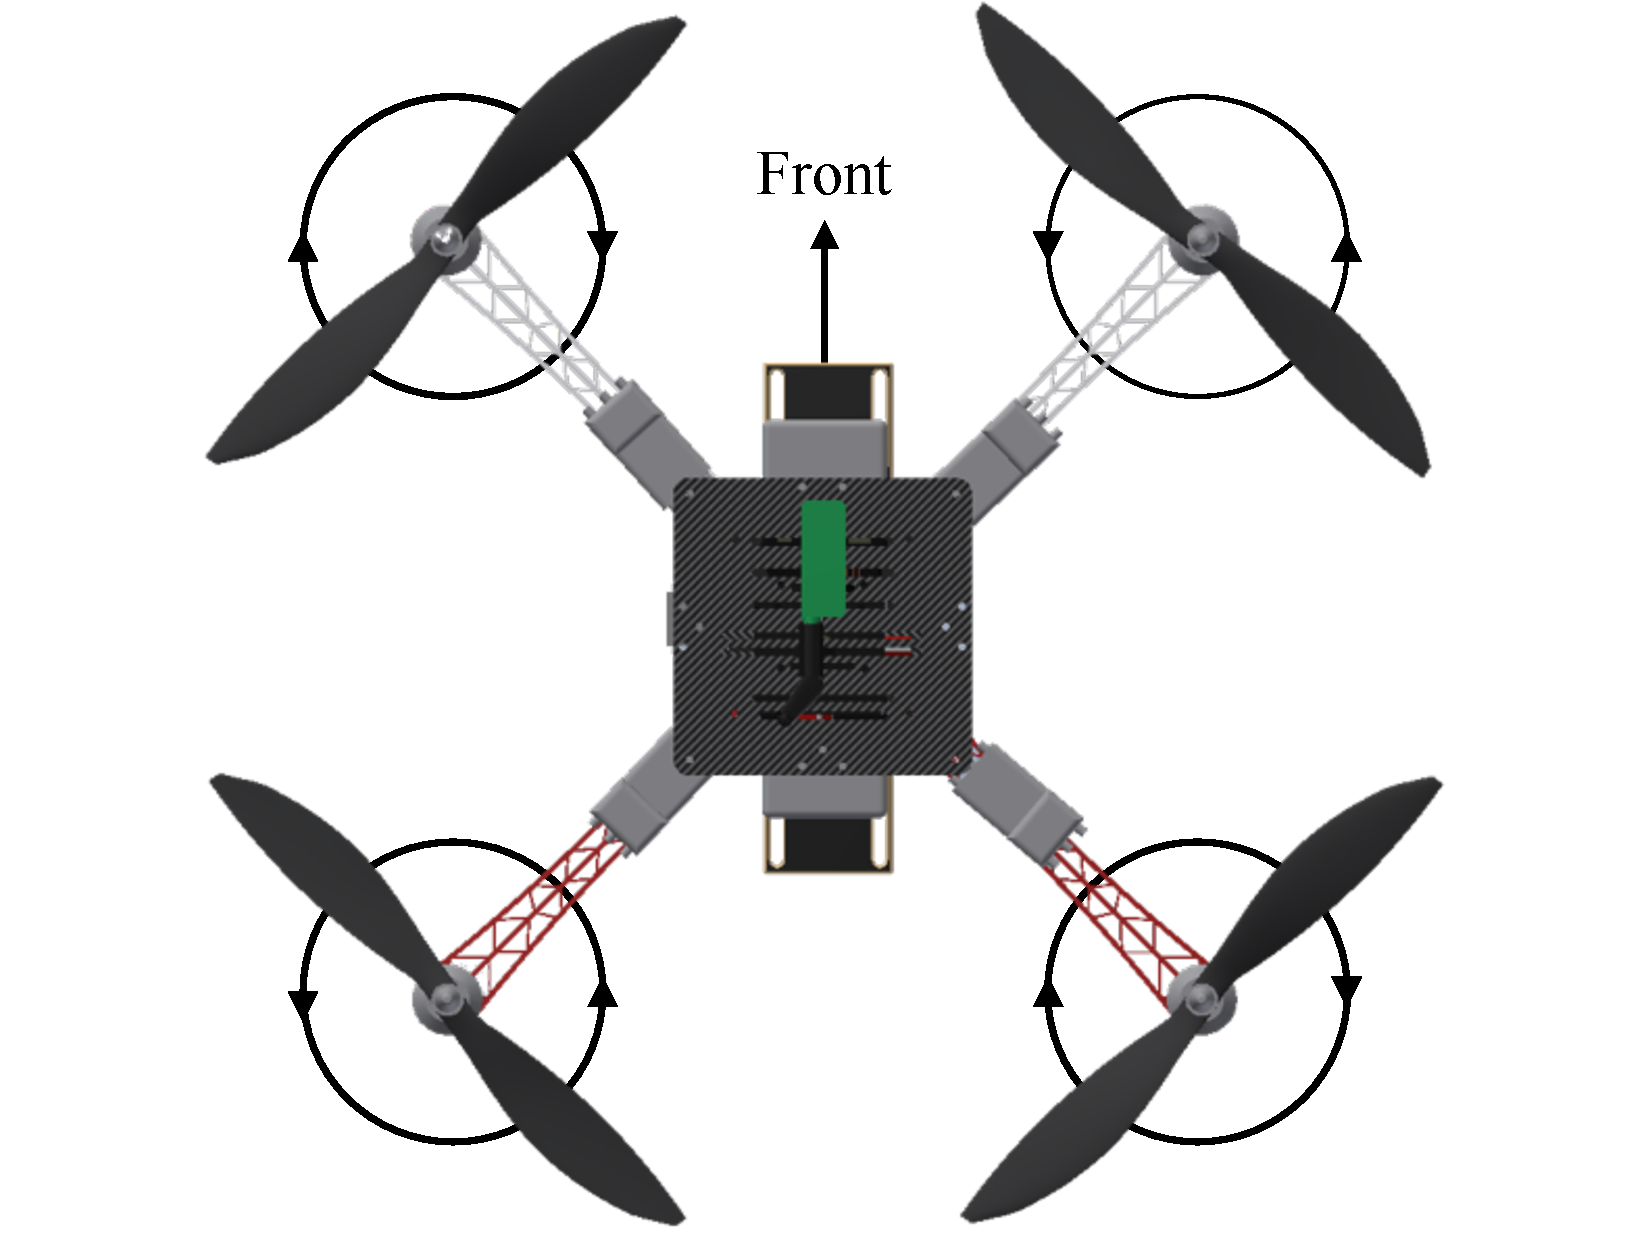
\includegraphics[width=0.5\textwidth]{graphics/geometry.pdf}
    \caption{Illustration of the Quadrotor Frame and the Rotors}
    \label{fig:geometry}
\end{figure}

\subsection{Actuator Motors} 

A quadrotor controls its attitude and thrust by independent inputs of its four motors. AC2830-358 850kV Brushless DC motors developed by 3D Robotics are used in this research \cite{motor}. The maximum power of the motors is 187 W. Since we use brushless DC motors, the quadrotor requires ESCs to run the motors. ESCs are also developed by 3D Robotics \cite{esc}. Power is provided to each motor by an 11.1V 2700mAh 3-cell lithium polymer battery. A motor rotates at a frequency corresponding to its voltage, and the average voltage of a motor can be controlled by Pulse Width Modulation (PWM). Details of motor control are stated in Section 3.5. Each motor spins a propeller, providing thrust and moment to each motor.

\begin{figure}
    \centering
    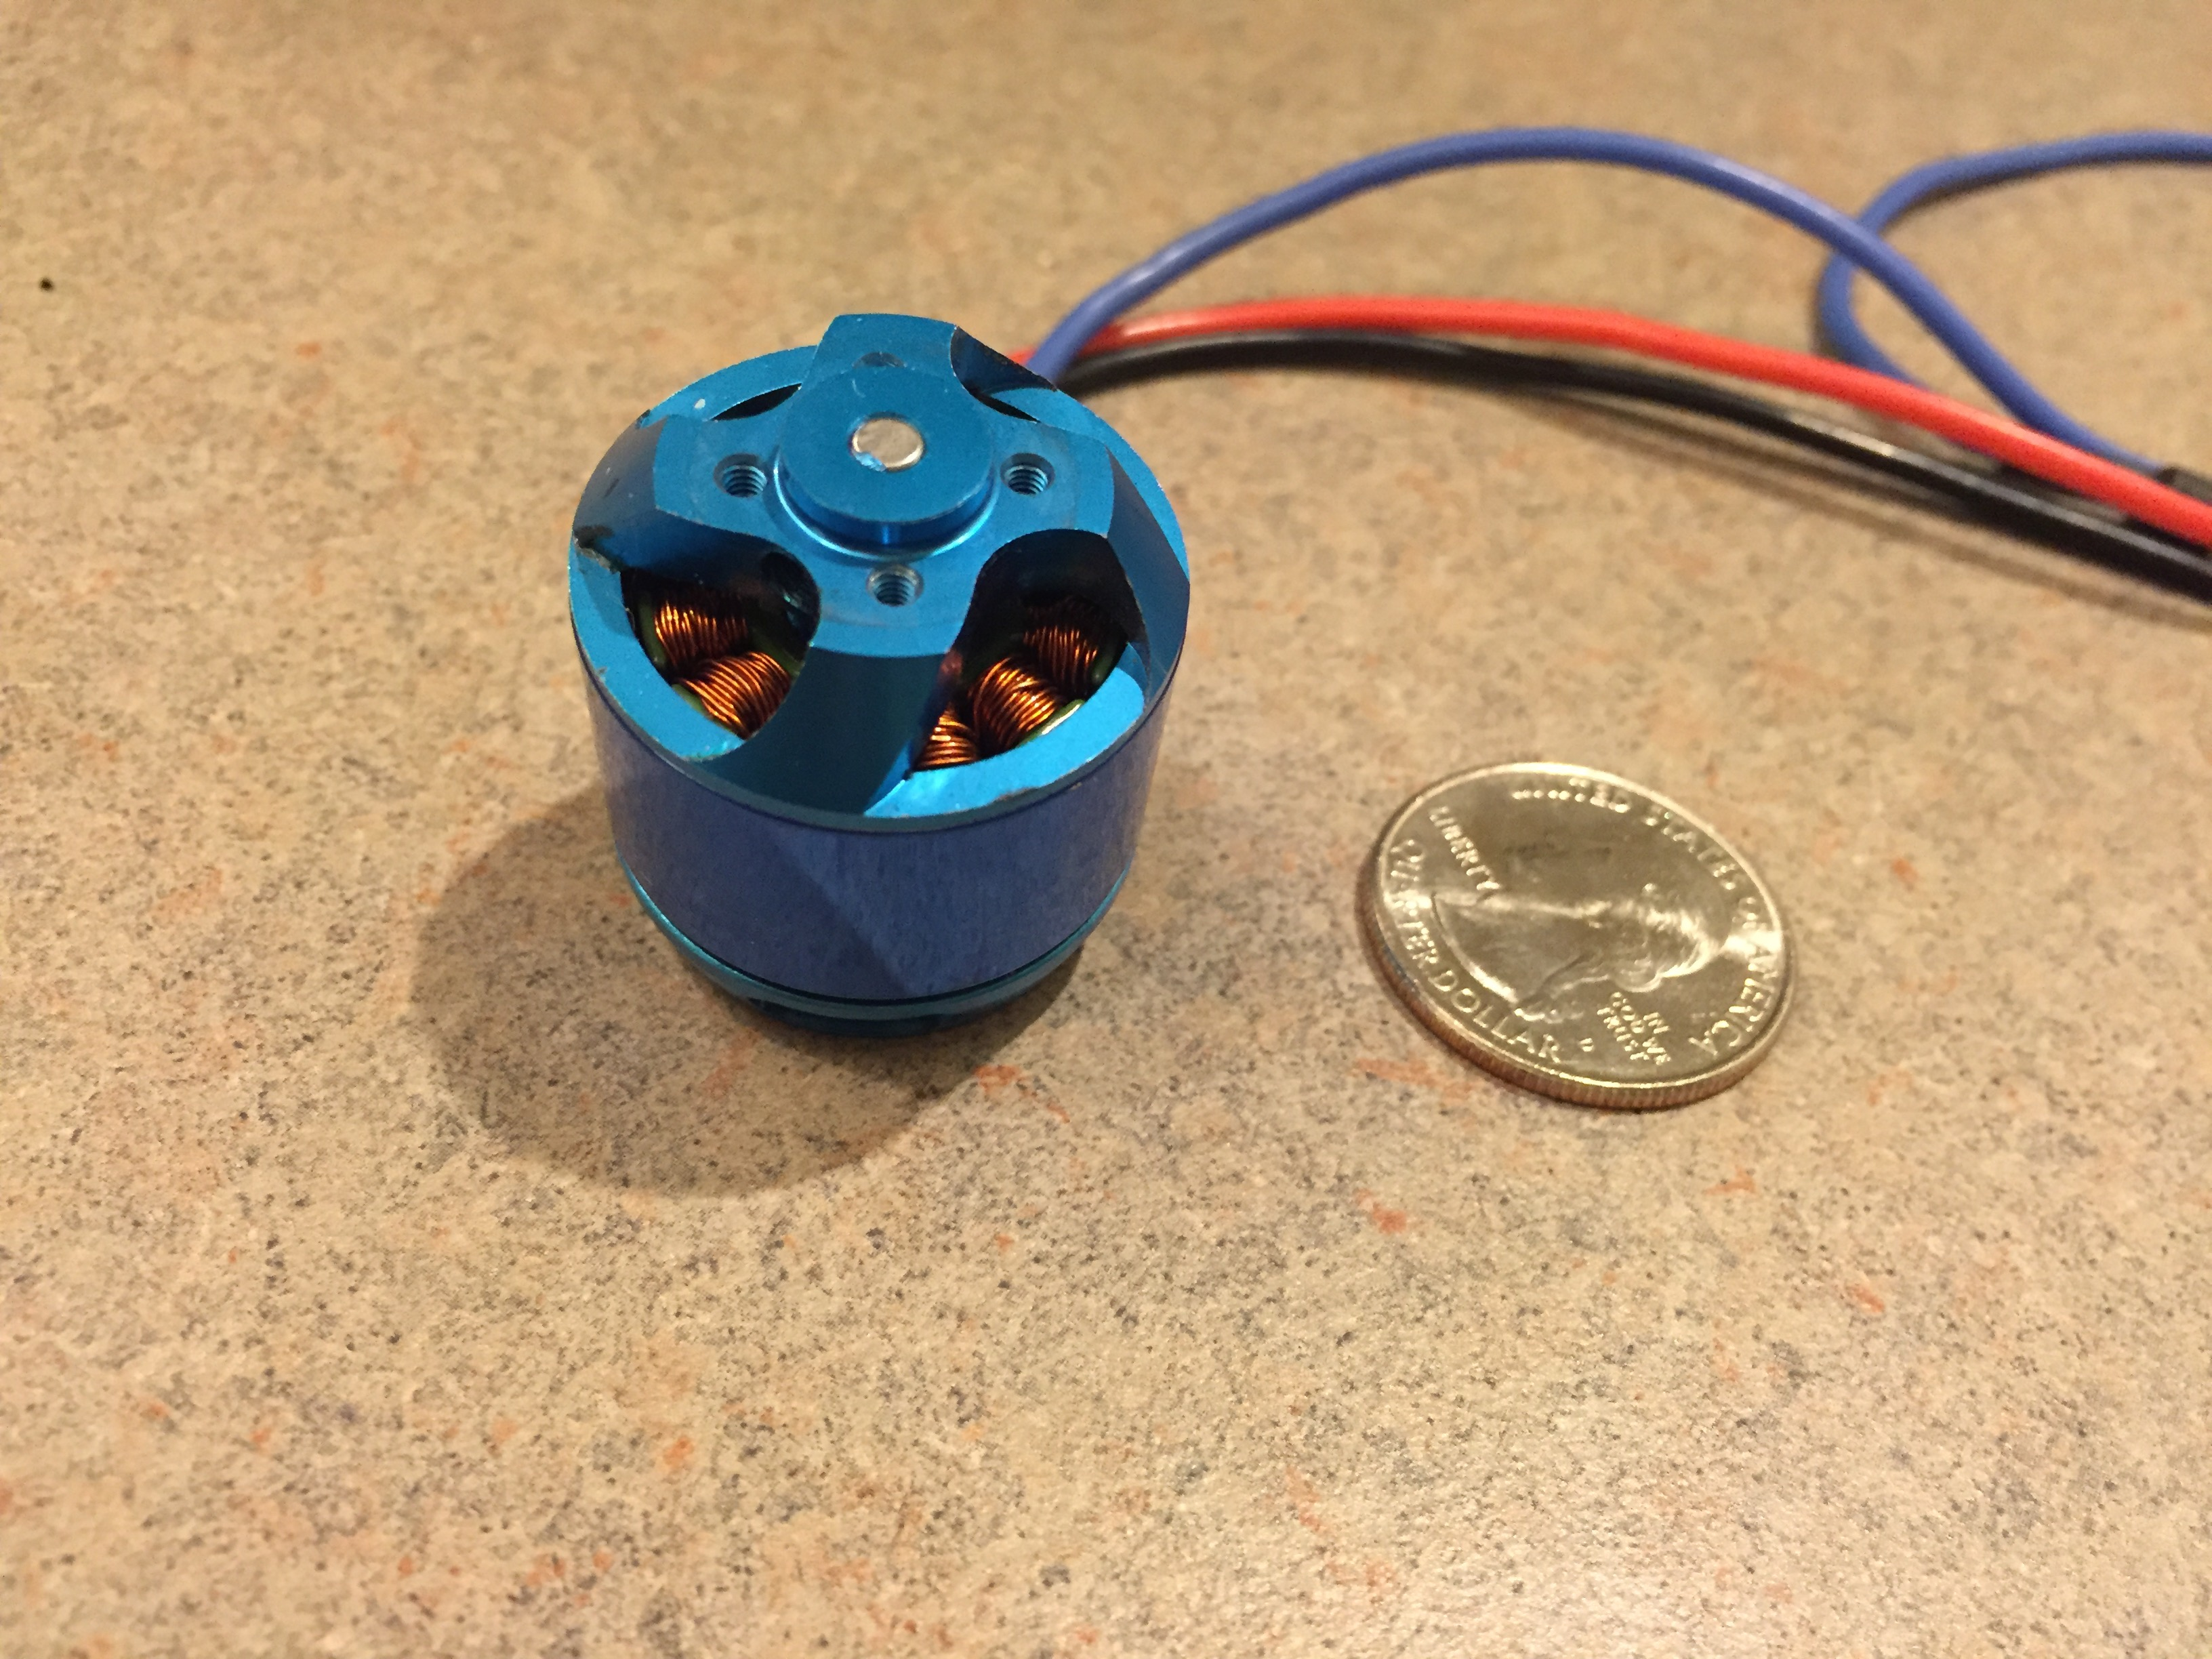
\includegraphics[width=0.5\textwidth]{graphics/motor.jpg}
    \caption{Brushless DC Motor}
    \label{fig:motor}
\end{figure}

\begin{figure}
    \centering
    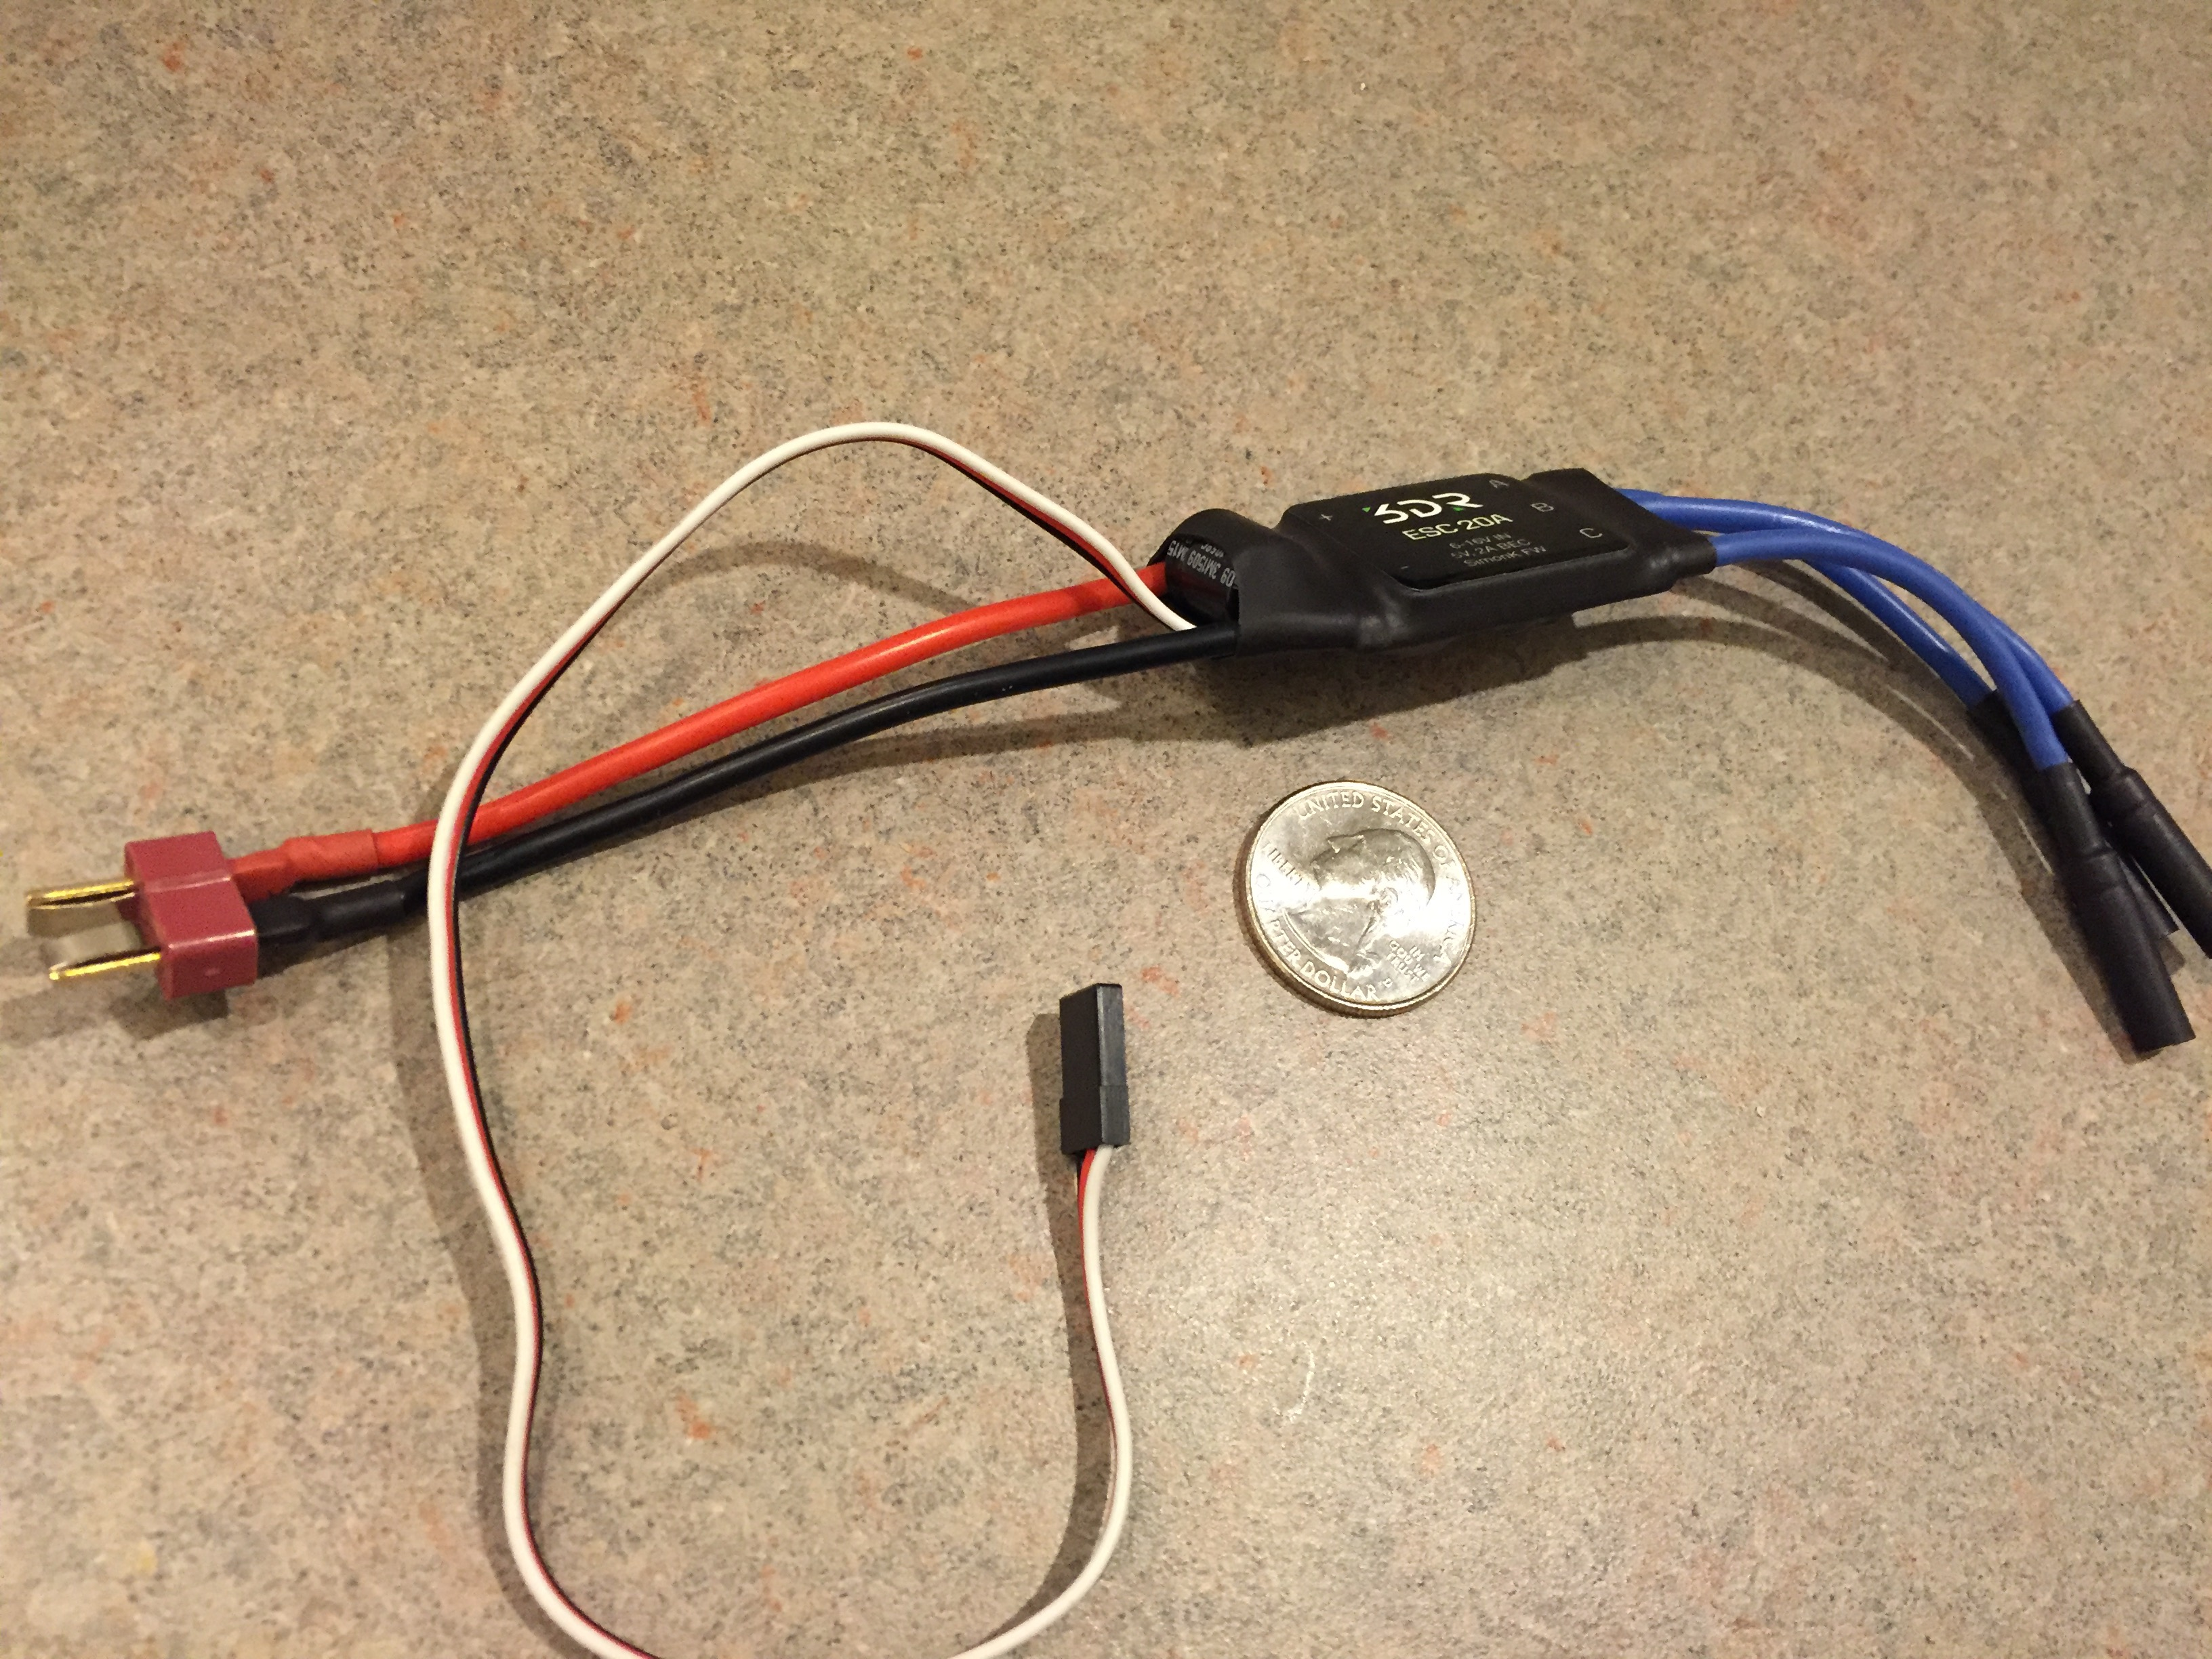
\includegraphics[width=0.5\textwidth]{graphics/esc.jpg}
    \caption{Electric Speed Control (ESC)}
    \label{fig:esc}
  \end{figure}
  
\begin{figure}
    \centering
    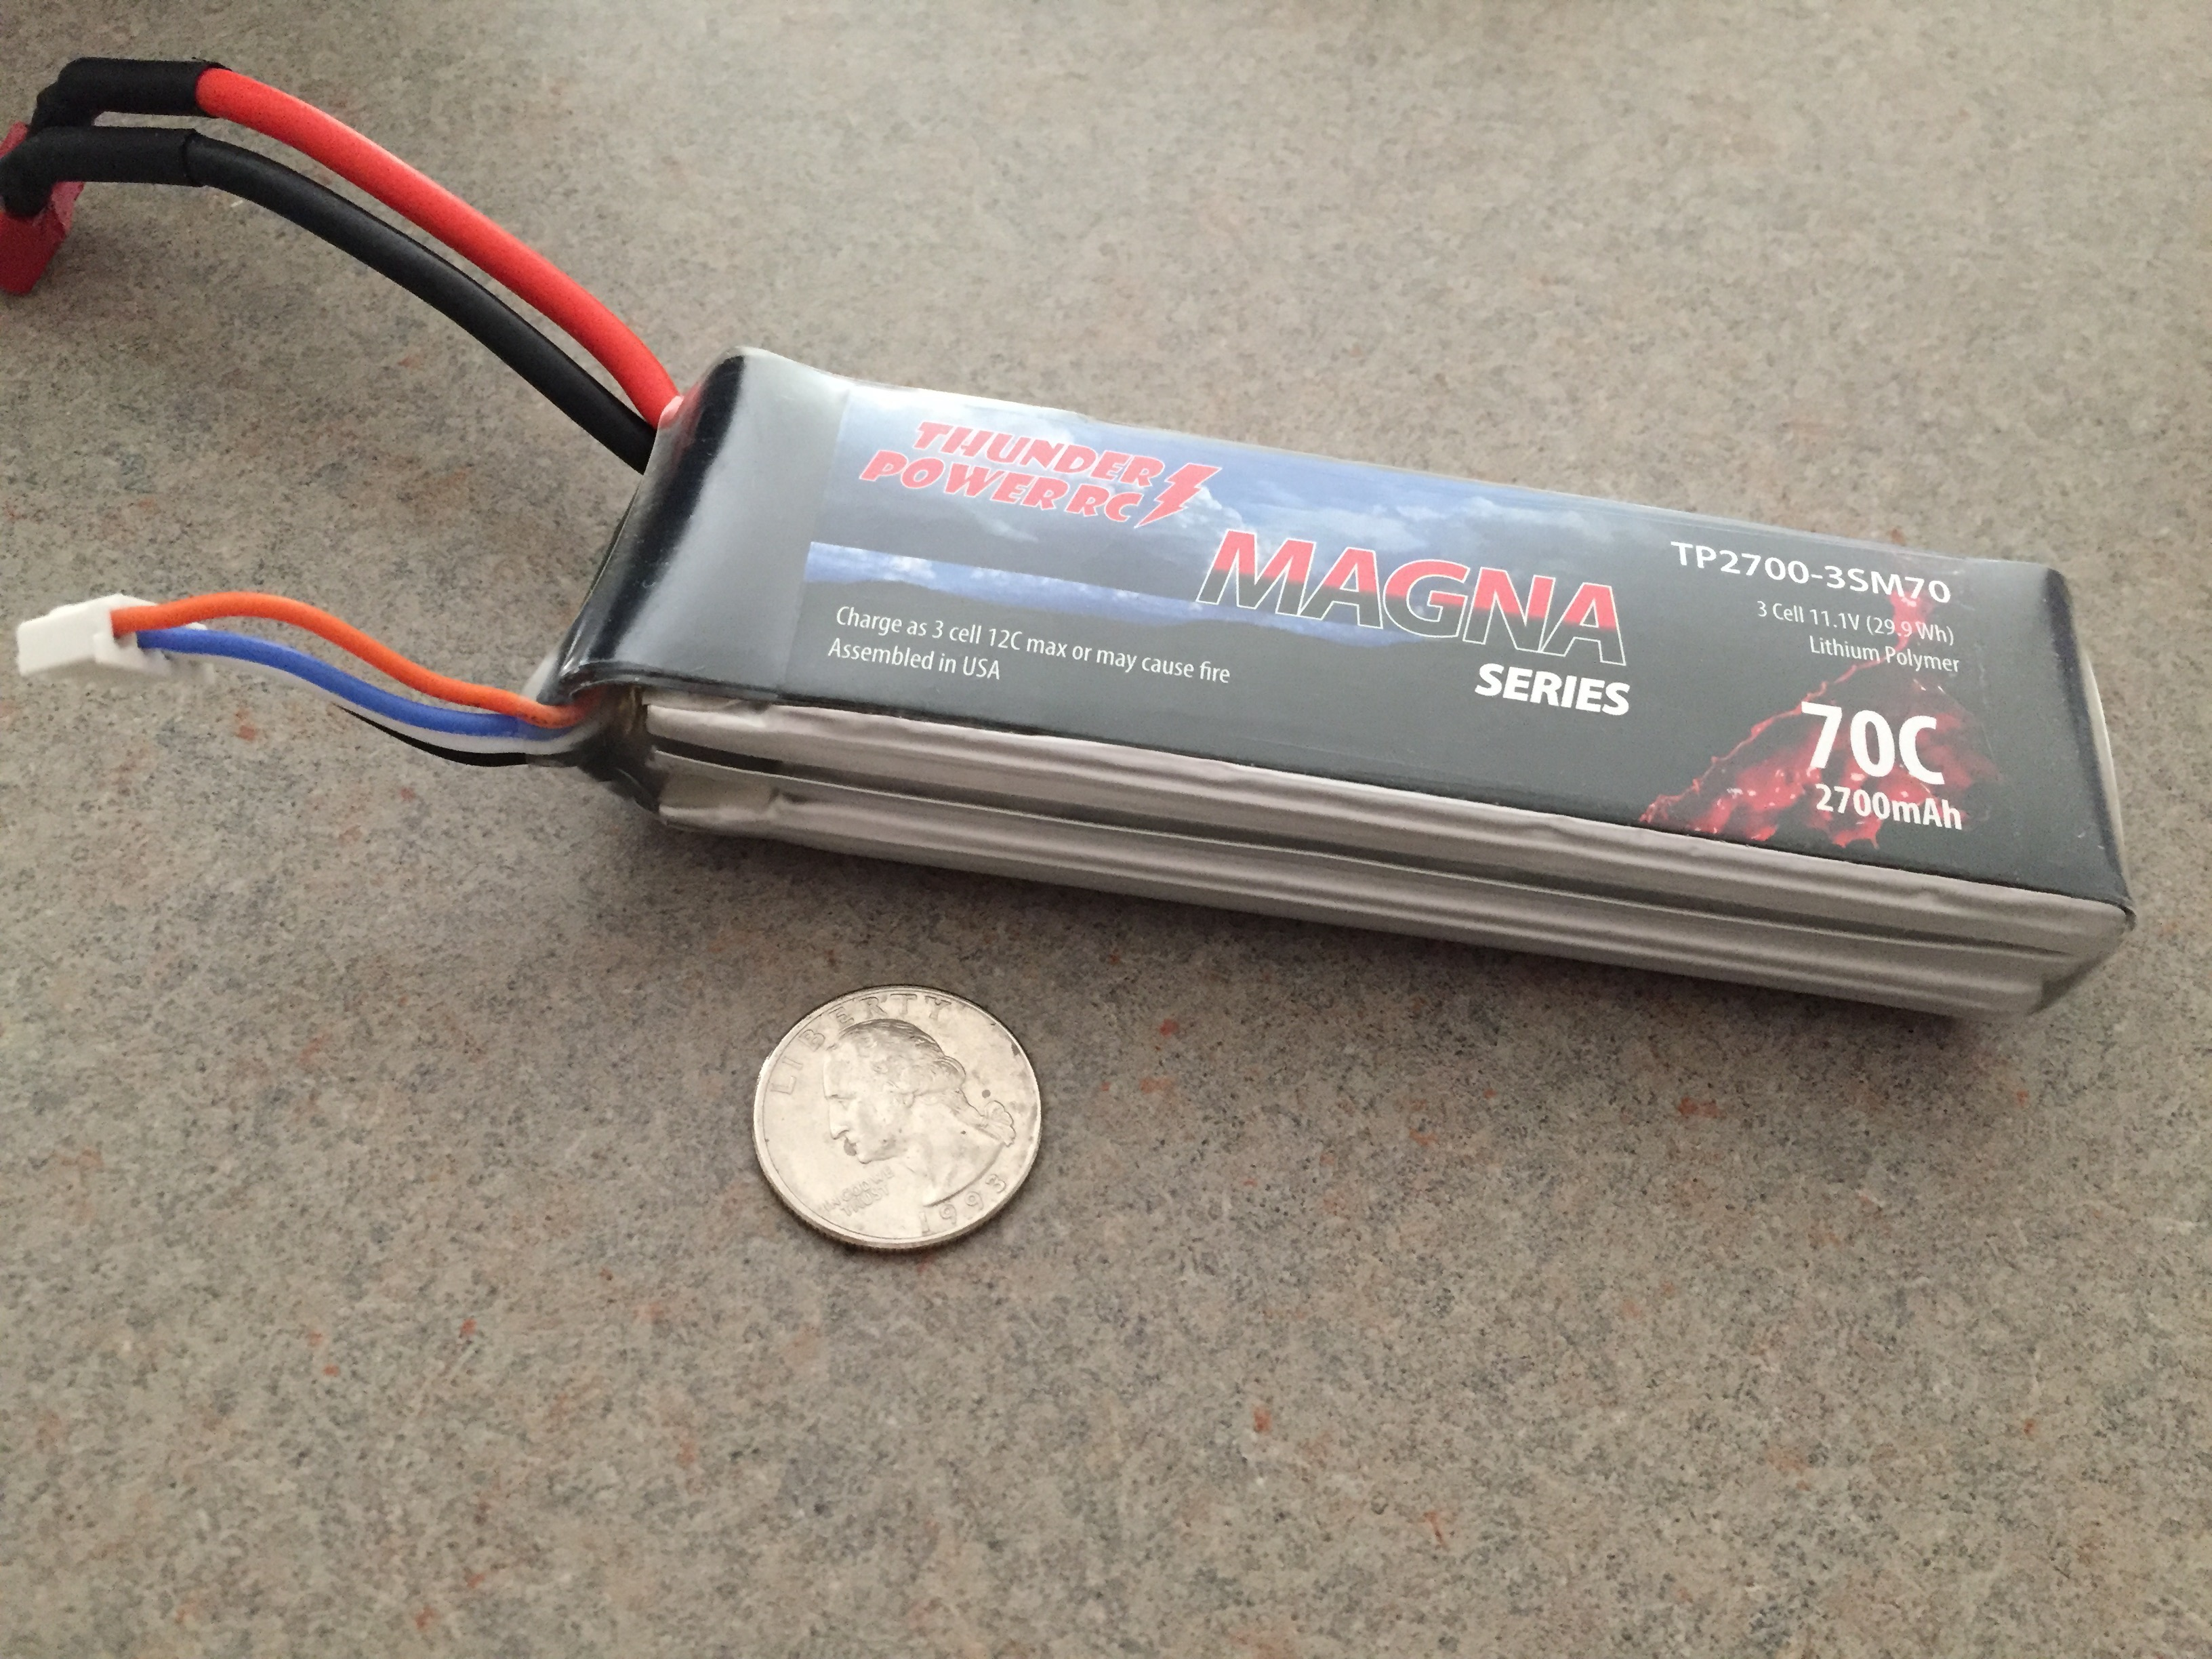
\includegraphics[width=0.5\textwidth]{graphics/battery.jpg}
    \caption{11.1V 2700mAh LiPo Battery}
    \label{fig:battery}
 \end{figure}
 
\subsection{Propeller}

In the quadrotor, two pairs of propellers, APC \(10 \times 4.7\) Slow Flyer (SF) and Slow Flyer Pusher (SFP) propellers, developed by APC Propellers Company, are used \cite{apc}. Both SF and SFP propellers have same geometries as shown at table \ref{table:propeller} but are mirror symmetric to each other. SF propellers are designed to rotate clockwise and SFP propellers are designed to rotate counter-clockwise. As shown in Figure \ref{fig:geometry}, the front-right and rear-left rotors rotate counter-clockwise with SF propellers, and the front-left and rear-right rotors rotate clockwise with SFP propellers. The weight of each propeller is measured as 0.012 kg.

\begin{table}[h]
\begin{center}
\begin{tabular*}{0.85\textwidth}{@{\extracolsep{\fill} } | c | r | r | r | r | }
  \hline
  & 						Entire Diameter &	Hub Diameter &	Hub Thickness &	Shaft Diameter \\
  \hline 
  Length [\(10^{-2} \text{m}\)] & 	{25.4} &		1.27  &			0.74  &			0.64  \\
  \hline
\end{tabular*}
  \caption{Geometry of APC \(10 \times 4.7\) Slow Flyer \cite{airfoil}}
  \label{table:propeller}
\end{center}
\end{table}

\begin{figure}
    \centering
    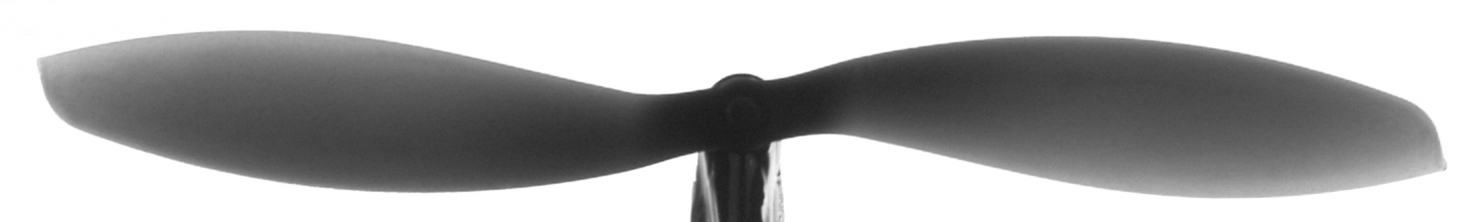
\includegraphics[width=0.8\textwidth]{graphics/apc10x47.jpg}
    \caption{APC  \(10 \times 4.7\) Slow Flyer \cite{airfoil}}
    \label{fig:propeller}
\end{figure}

\subsection{Autopilot}

A quadrotor is typically equipped with a microcontroller autopilot that is controlled by high level commands, such position or attitude setpoints from an RC transmitter. Based on the current state and setpoint commands, the controller computes desired actuation and commands the actuators to respond accordingly. In order to detect the current state, the autopilot requires an accelerometer, gyroscope, and some form of actuator interface in order to function. Since most autopilot systems use a PID controller to control attitude, it is necessary to rewrite the control algorithm. In order to facilitate this, we choose to use the open source PX4 autopilot system \cite{px4}. We used a 3D Robotics Pixhawk microprocessor to run our PX4 code \cite{3dr}. Pixhawk contains all the necessary sensors, computation power, and input/output interfaces. In addition to an accelerometer and a gyroscope, the Pixhawk has a magnetometer and barometer to measure altitude and attitude changes \cite{pixhawk}.

\begin{figure}
    \centering
    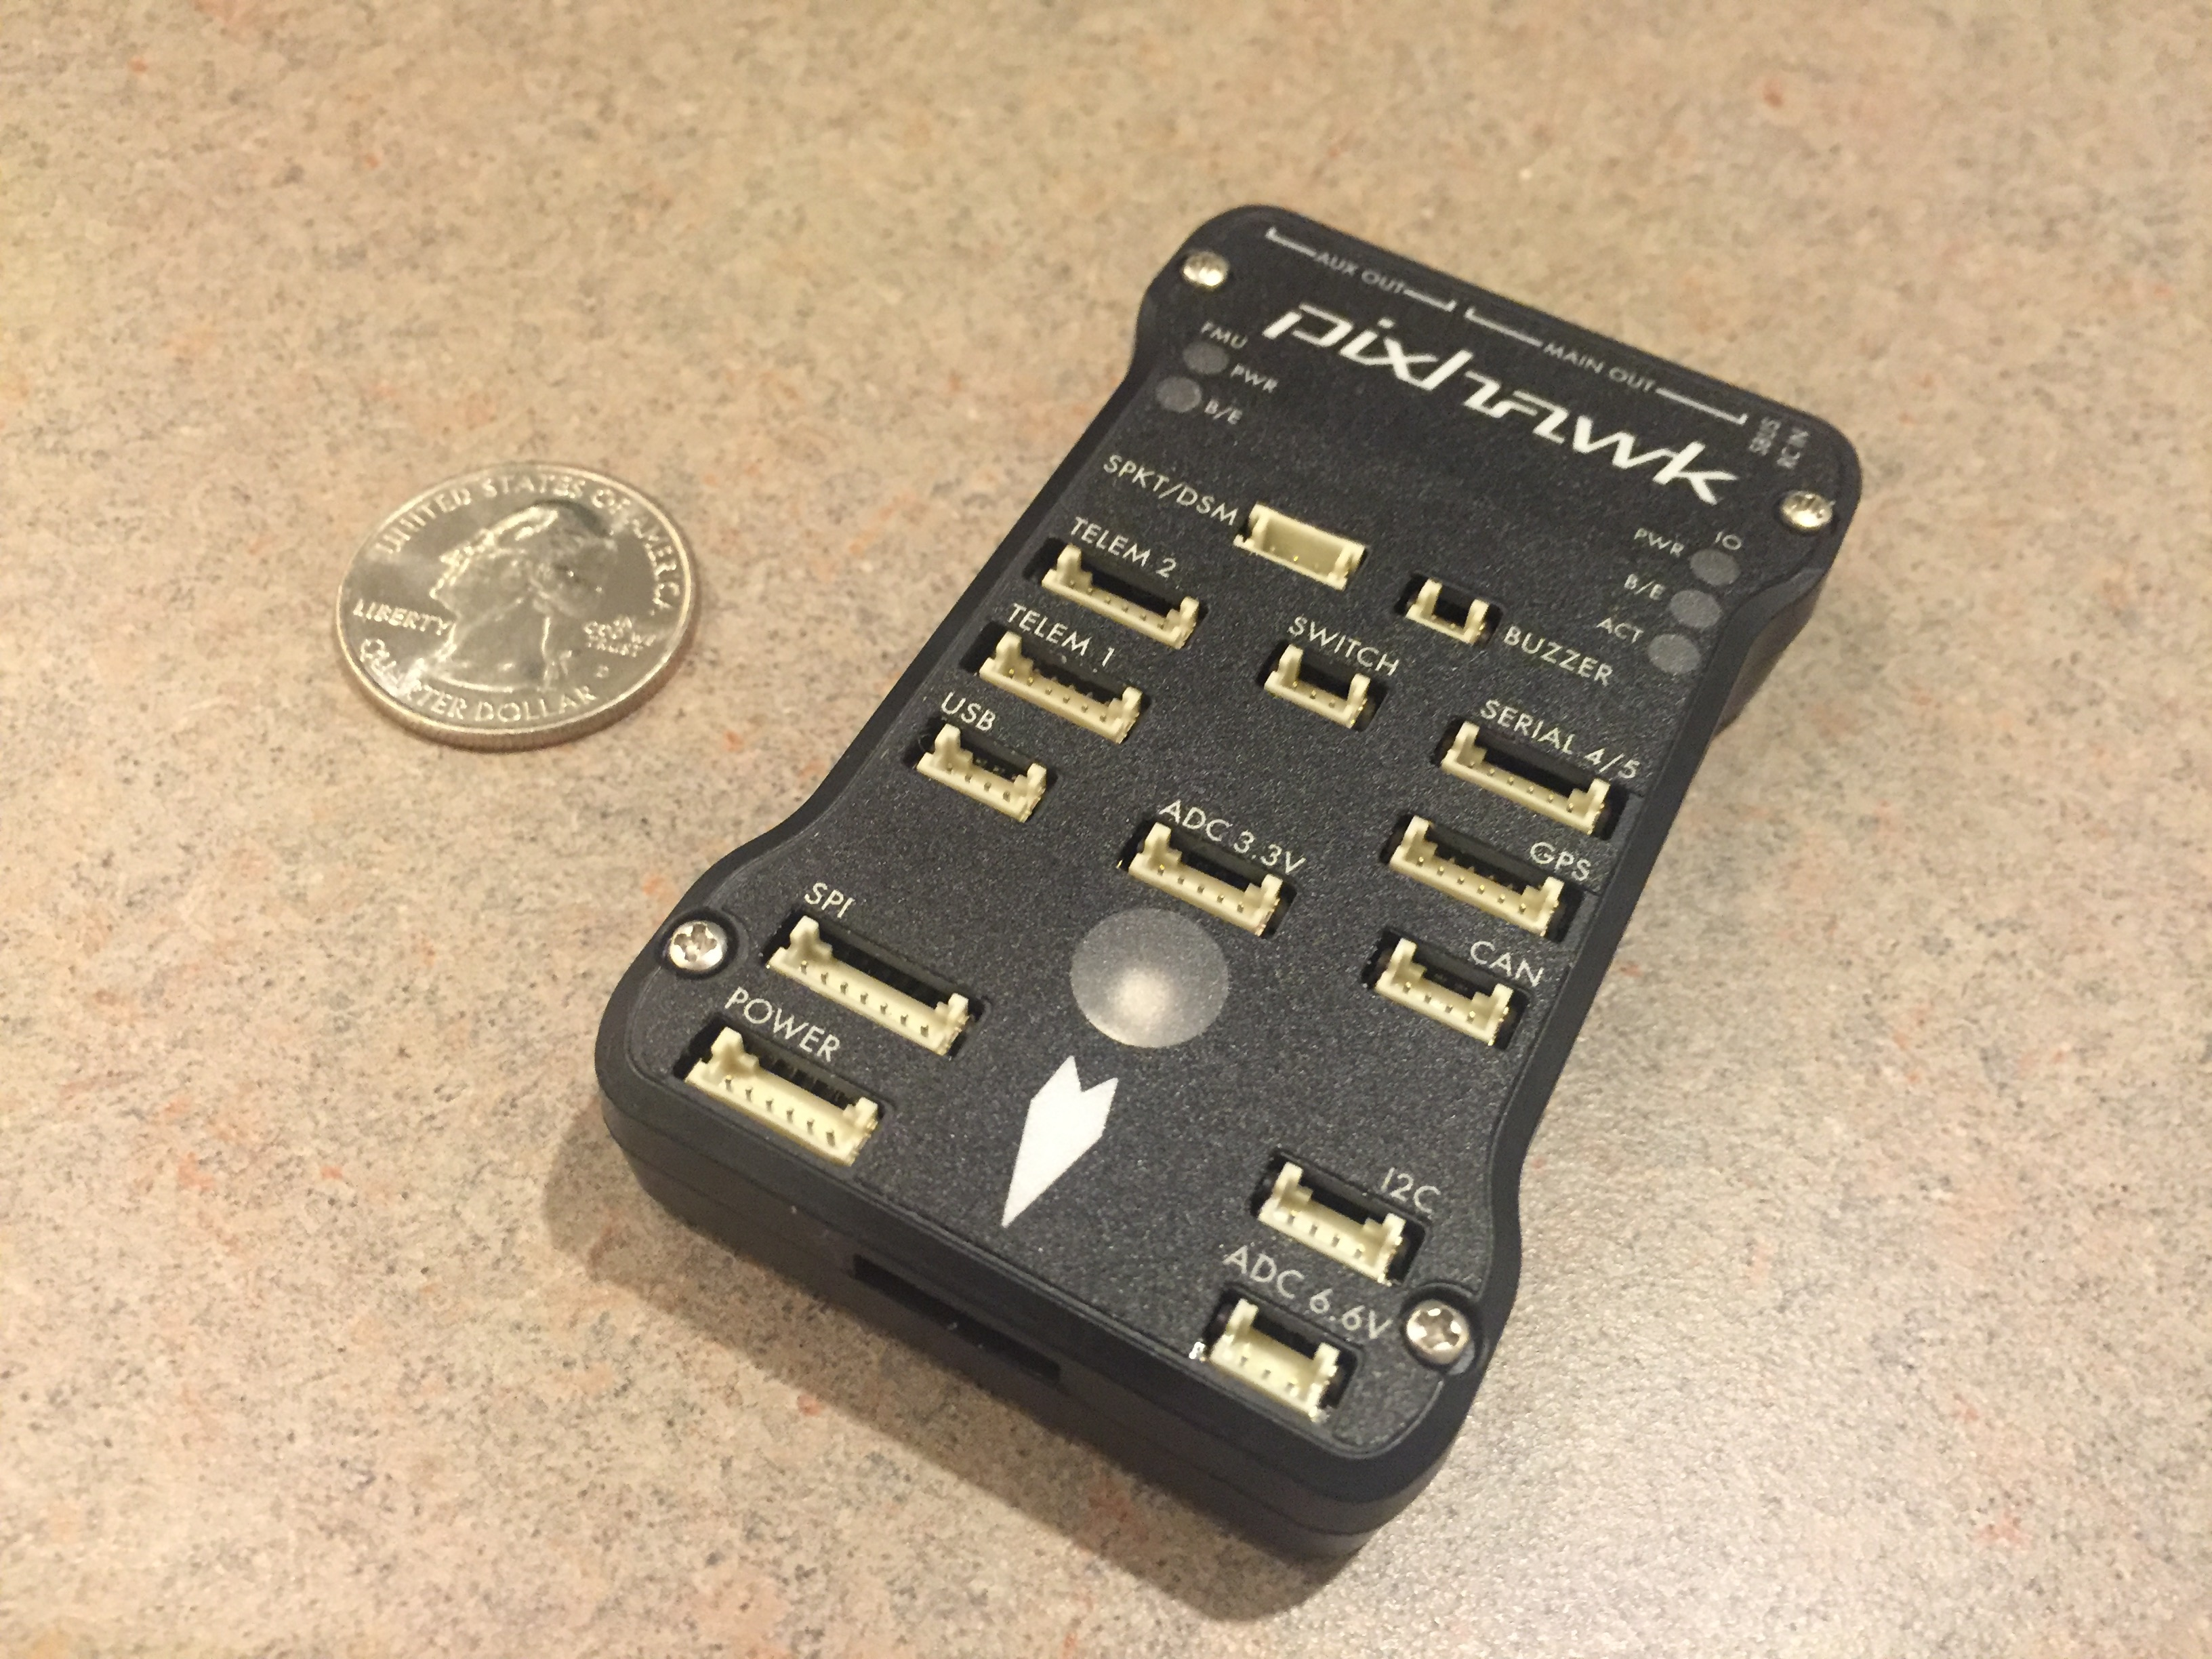
\includegraphics[width=0.5\textwidth]{graphics/pixhawk.jpg}
    \caption{Pixhawk Autopilot}
    \label{fig:pixhawk}
\end{figure}

\subsection{Companion Single-Board Computer}

The companion computer is necessary for estimating the quadrotor position through computer vision. The computer receives image data from a ground facing camera and, using the quadrotor state from the autopilot, computes the position estimation of the quadrotor and sends the estimation data to the autopilot. The quadrotor uses a single Hardkernel Odroid XU4 \cite{hardkernel}. It is a quadcore 1.3 GHz CPU and 2 GB of RAM. The computer runs on a 5 volt 4 amp power supply, which is provided by a voltage converter from the main battery.

\begin{figure}
    \centering
    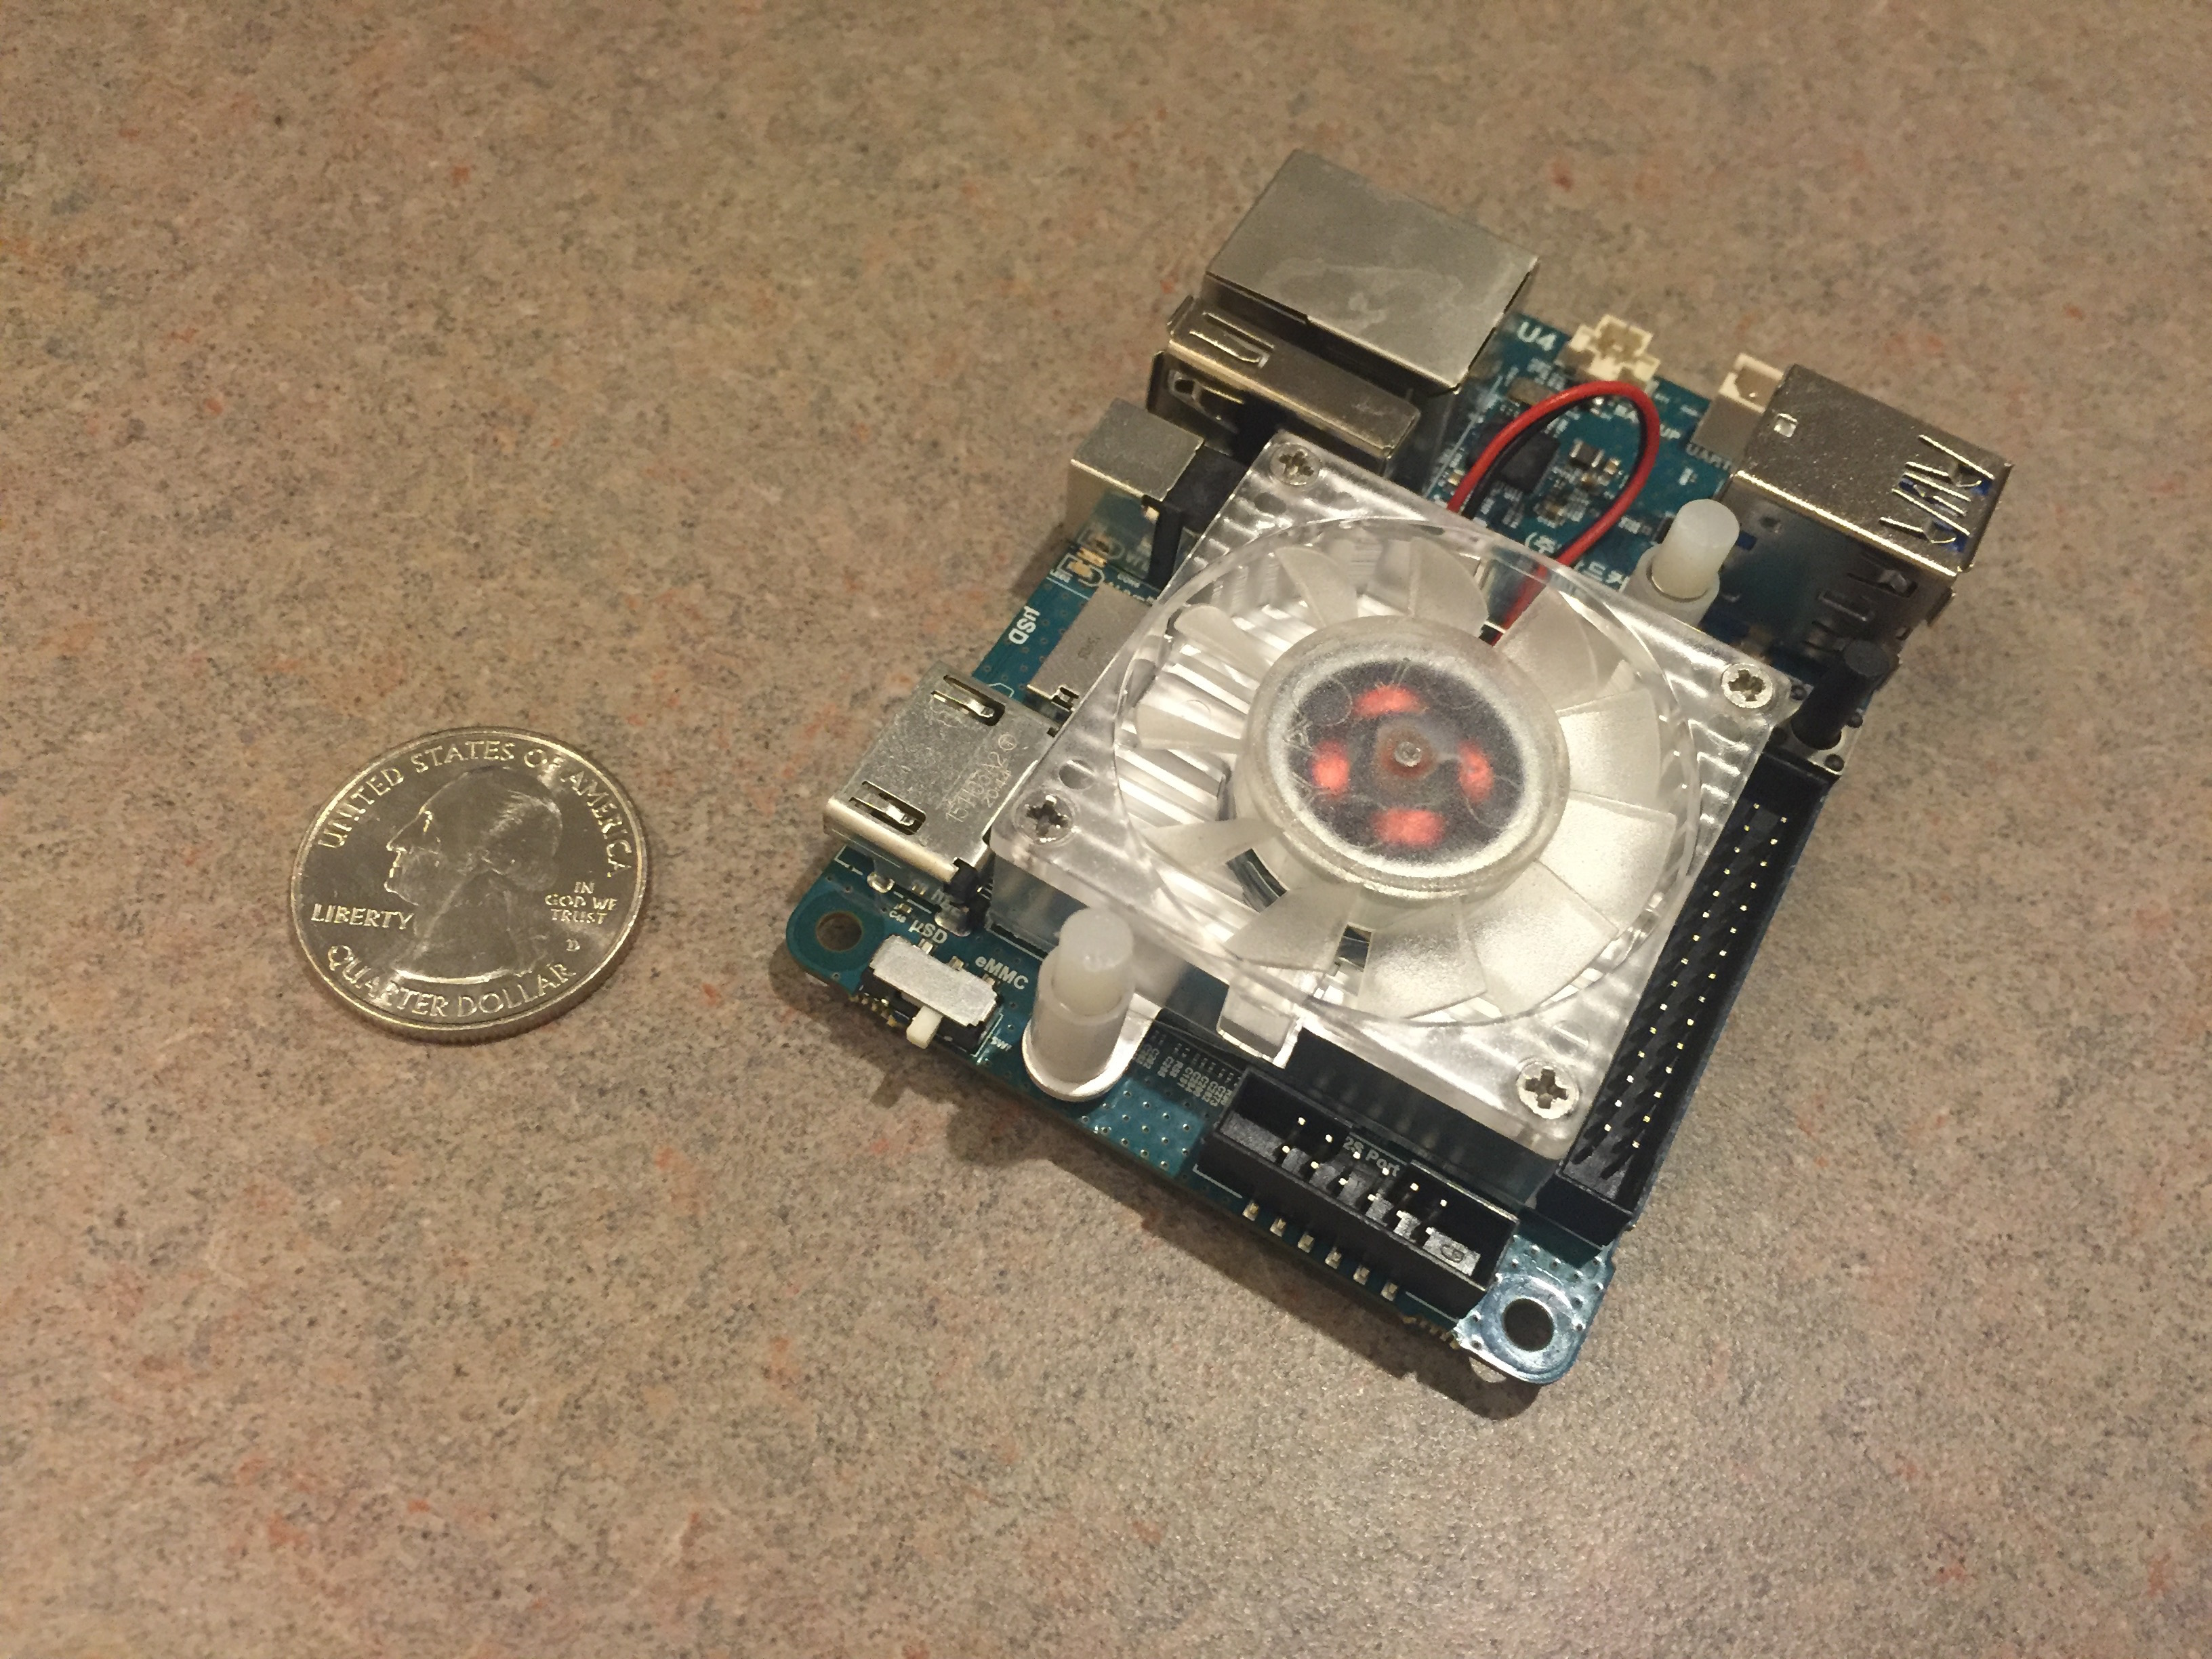
\includegraphics[width=0.5\textwidth]{graphics/odroid.jpg}
    \caption{Odroid XU4 Single-board Computer}
    \label{fig:odroid}
\end{figure}

\subsection{Camera}

The autopilot does not have precise position measurement, so it is necessary to estimate the quadrotor's position precisely using a computer vision system. Four circular markers on the floor are tracked by the quadrotor's camera to provide estimates as to its relative position with respect to the markers. A ground facing camera is used to capture the images of the markers. The USB webcam we use has a focal length of 2.1mm and has about \({120}^{\circ}\) view angle. The camera sends images of \(640 \times 480\) pixels at a rate of 30 frames per second. This sensor is used for vision-based estimation presented in Chapter 5.

\begin{figure}
    \centering
    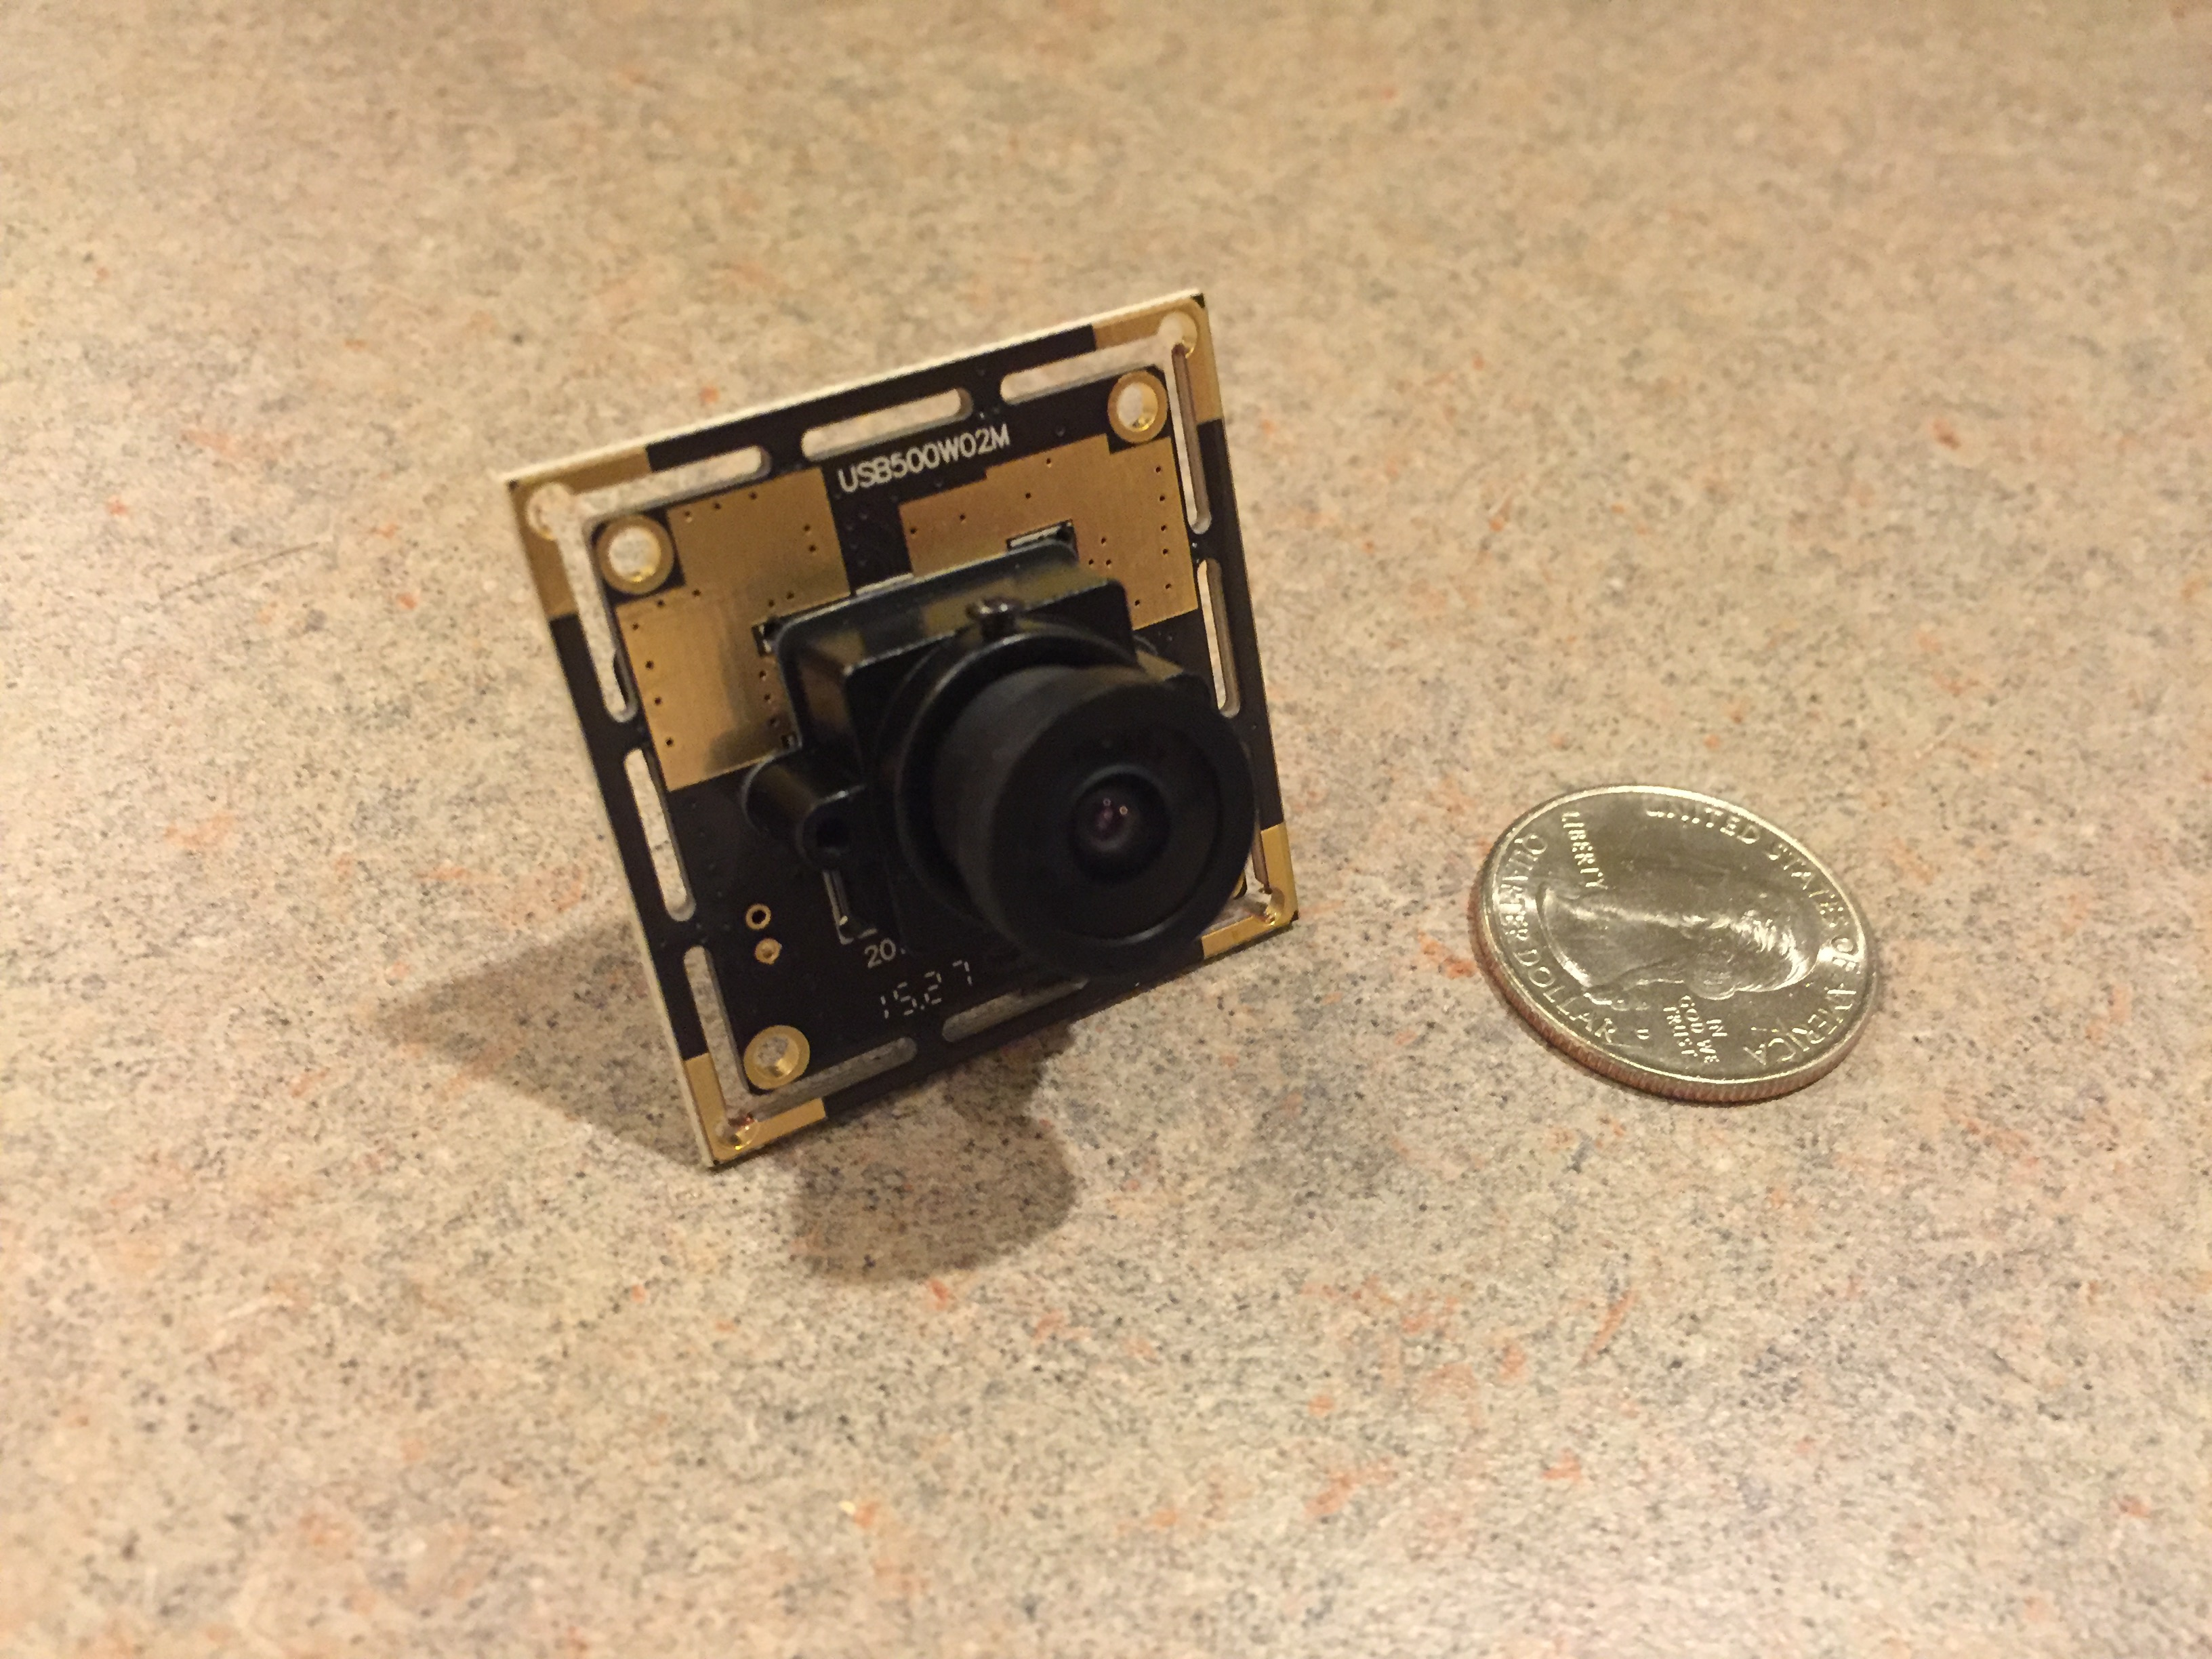
\includegraphics[width=0.5\textwidth]{graphics/camera.jpg}
    \caption{USB Camera}
    \label{fig:camera}
\end{figure}

\subsection{Wireless Communication Interface}

In the quadrotor system, two different communication methods are used. First, in the case of offboard control, bidirectional radio communication is used to exchange messages between a ground control station and the quadrotor, and unidirectional radio communication is used to send inputs from a human user using an RC transmitter. A pair of 3DR Radio V2 kits, developed by 3D Robotics, was used for the bidirectional radio communication, and an AR610 6-channel DSMX Aircraft Receiver, developed by Spektrum, is used for unidirectional communication \cite{radio}\cite{spektrum}. The communication for the ground control station uses 915 MHz frequency and the one for the RC transmitter uses 2.4 GHz frequency.

\begin{figure}
    \centering
    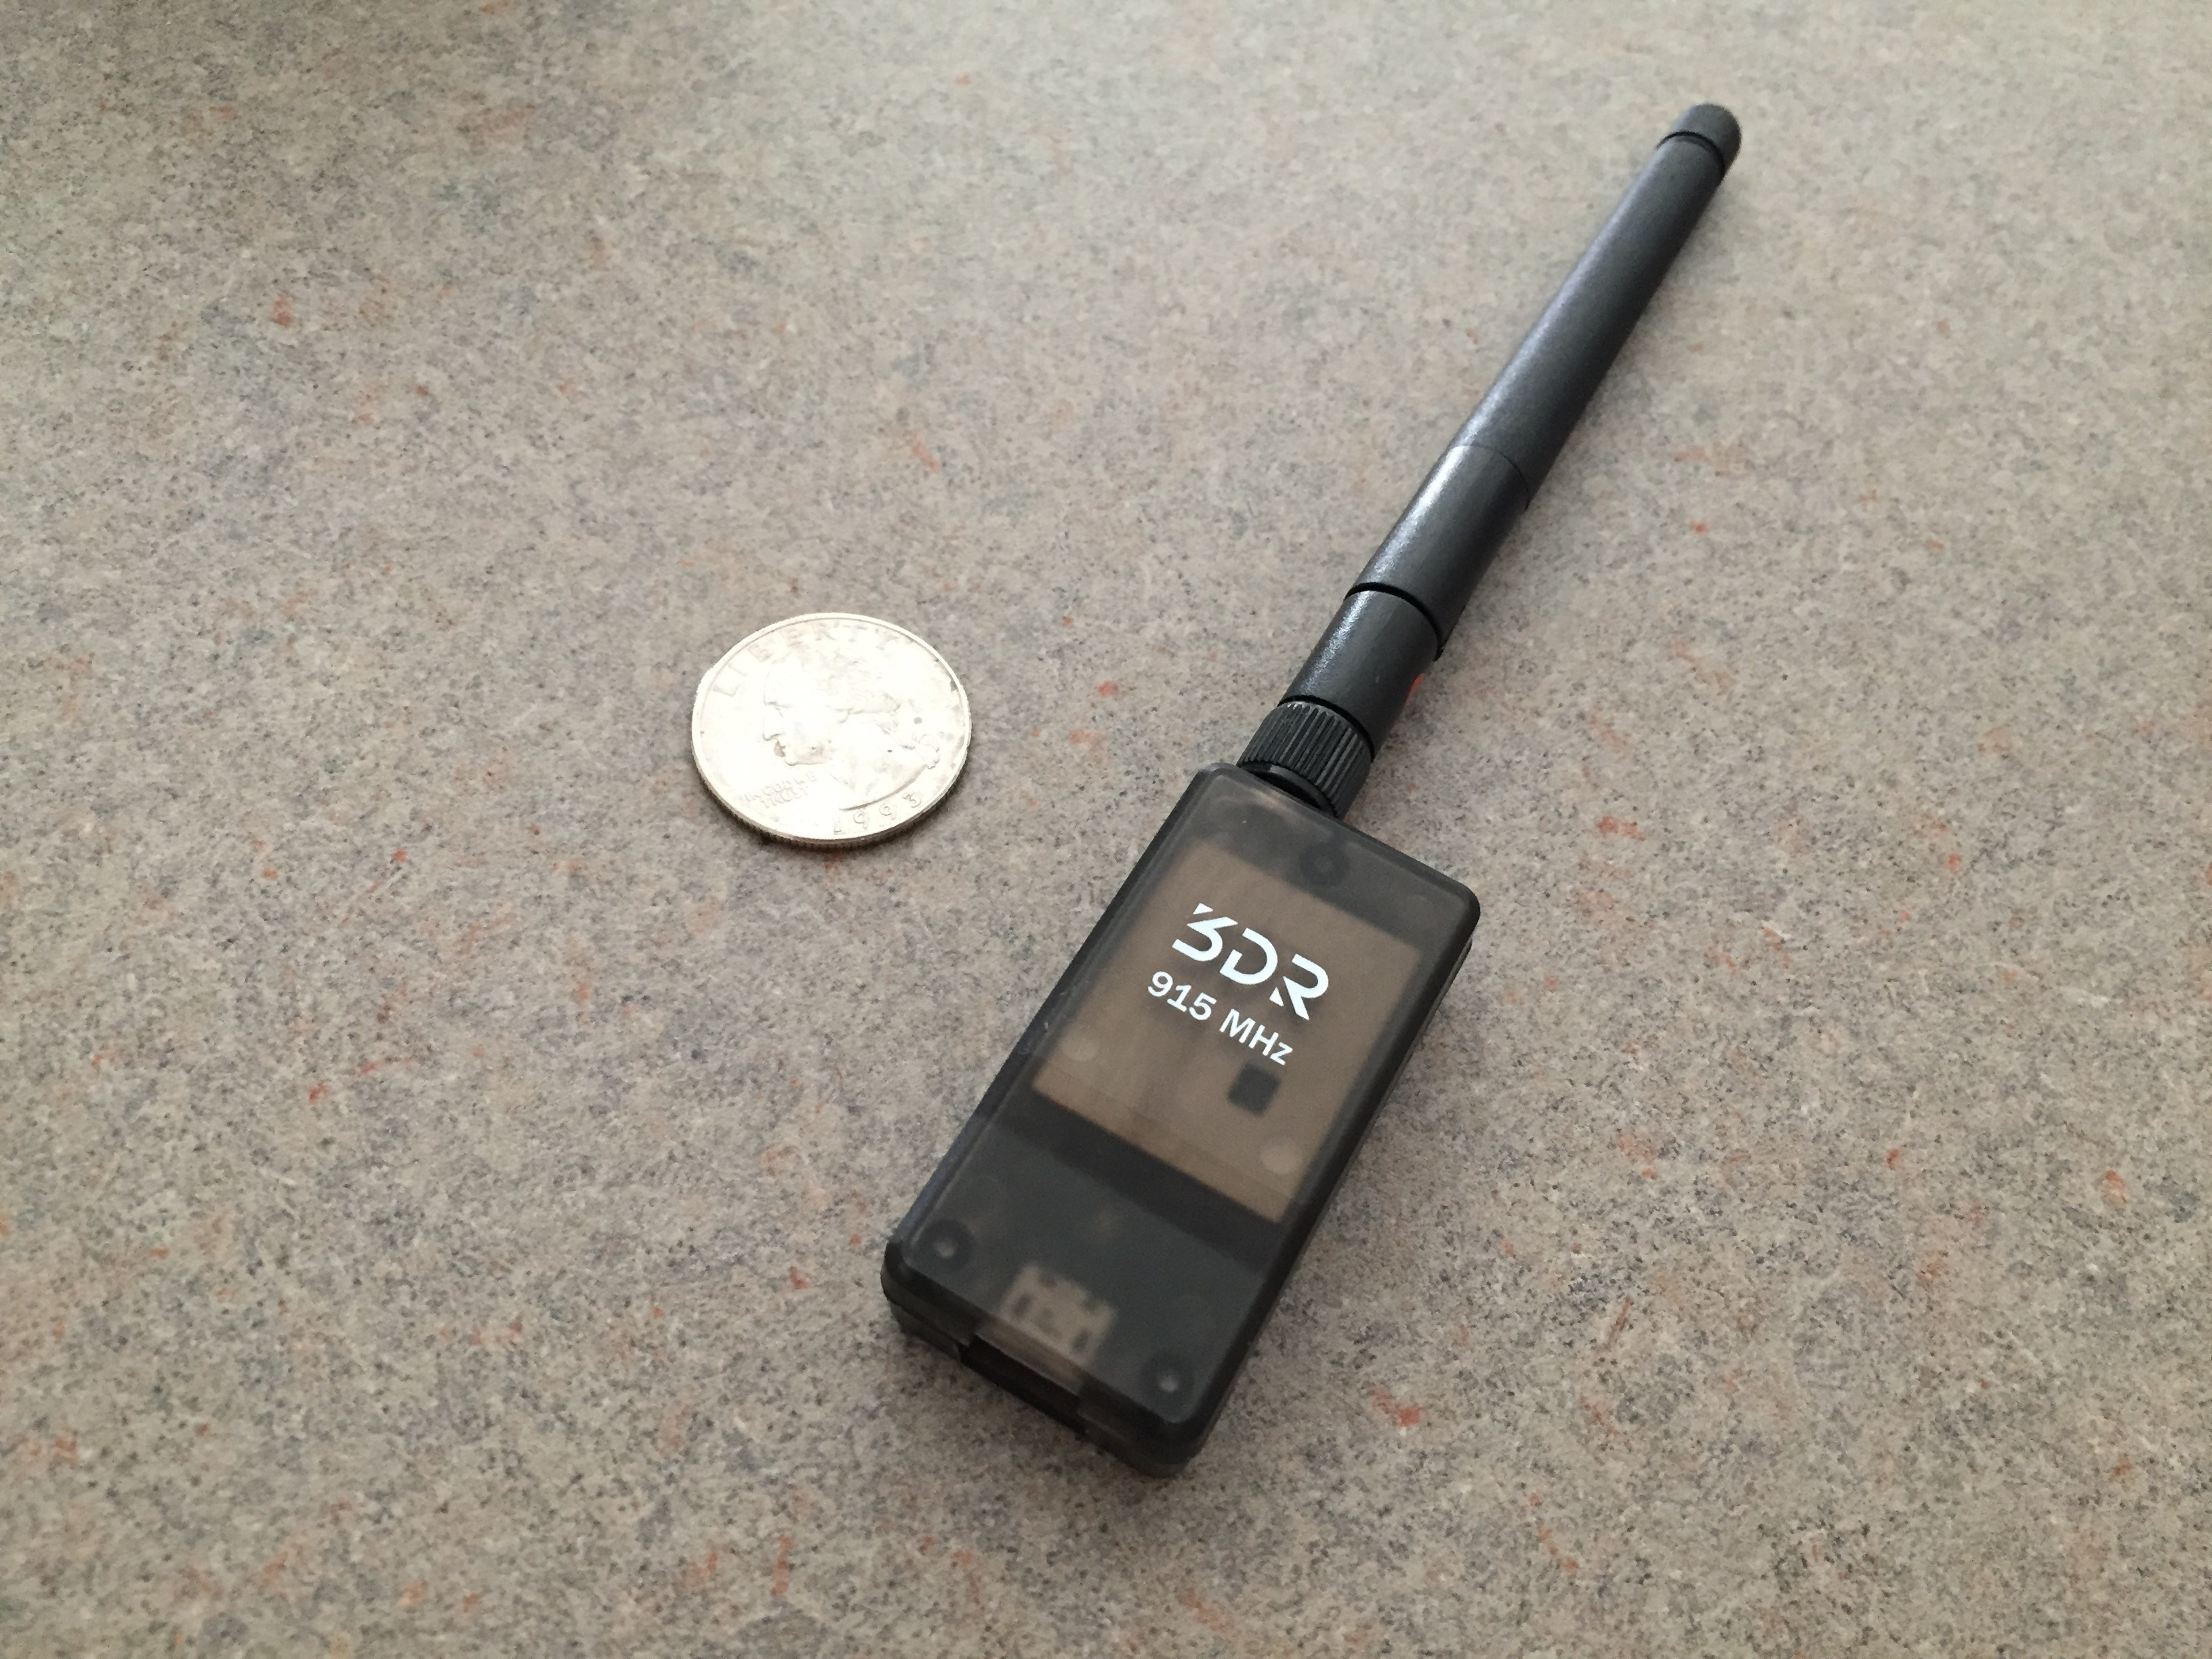
\includegraphics[width=0.5\textwidth]{graphics/telemetry.jpg}
    \caption{3DR radio V2 Telemtery}
    \label{fig:telemetry}
\end{figure}

\begin{figure}
    \centering
    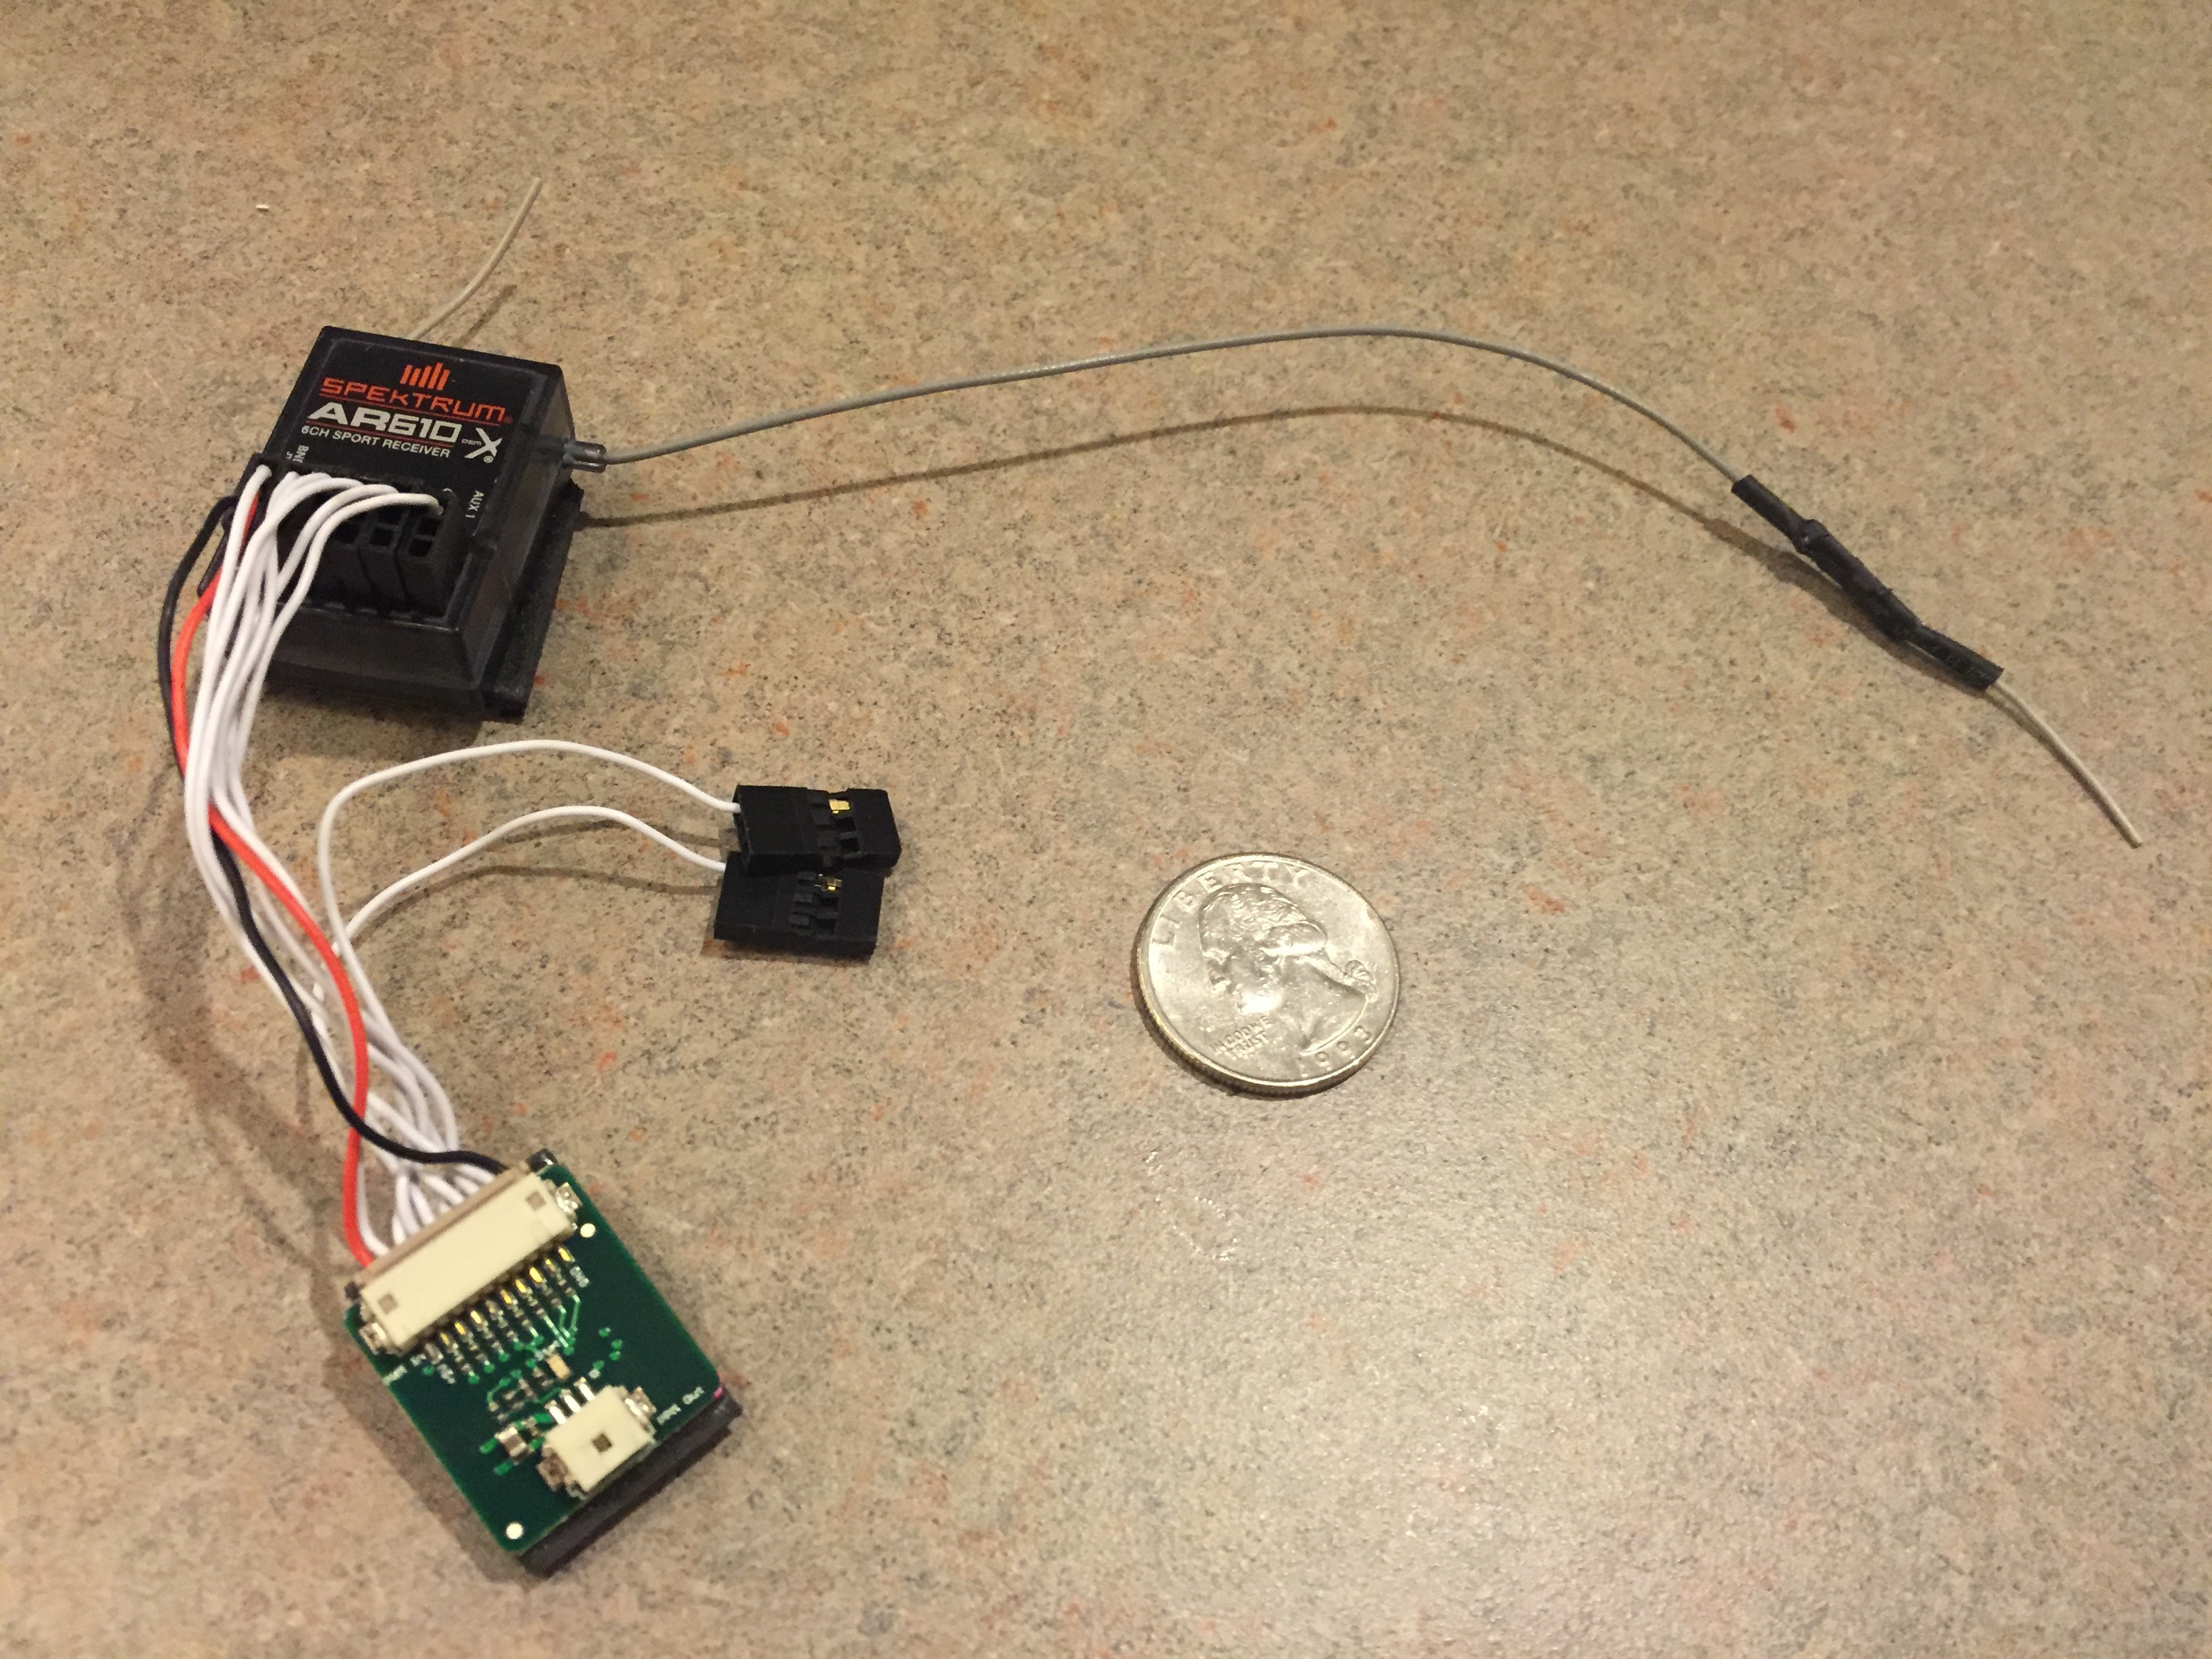
\includegraphics[width=0.5\textwidth]{graphics/rc.jpg}
    \caption{AR610 6-channel DSMX Aircraft Receiver}
    \label{fig:receiver}
\end{figure}

Secondly, in the case of onboard control, messages between the onboard computer and the autopilot are exchanged directly via wired serial communication, and a remote communication interface between the onboard computer and the ground control station is necessary instead. Therefore, a Wi-Fi network is used for communication between the onboard computer and the ground control station. The same communication between the quadrotor and the RC transmitter can be also used as backup. 

\subsection{Ground Control Station}

The ground control station allows us to send commands and receive data remotely. For offboard control, the ground control station must be connected with a radio telemetry with a proper baud rate to receive messages. The telemetry that is connected to the ground station computer must be paired with the one on the quadrotor. 

In the case of onboard control, any computer can be used as a ground control system so long as it is on the same Wi-Fi network since the quadrotor system uses the Wi-Fi network to communicate. The companion computer can be accessed using any wireless interface, such as SSH. Through this interface, a user can use the command console on the onboard companion computer remotely, and the quadrotor's operation can be started.

\section{System Overview}

The complete assembly of the quadrotor is shown in Figure \ref{fig:assemble_01} and \ref{fig:assemble_02}. An overview of the offboard systems of the quadrotor is shown in Figure \ref{fig:overview_01} and one of the onboard system for vision-based estimation is shown in Figure \ref{fig:overview_02}.

\begin{figure}
    \centering
    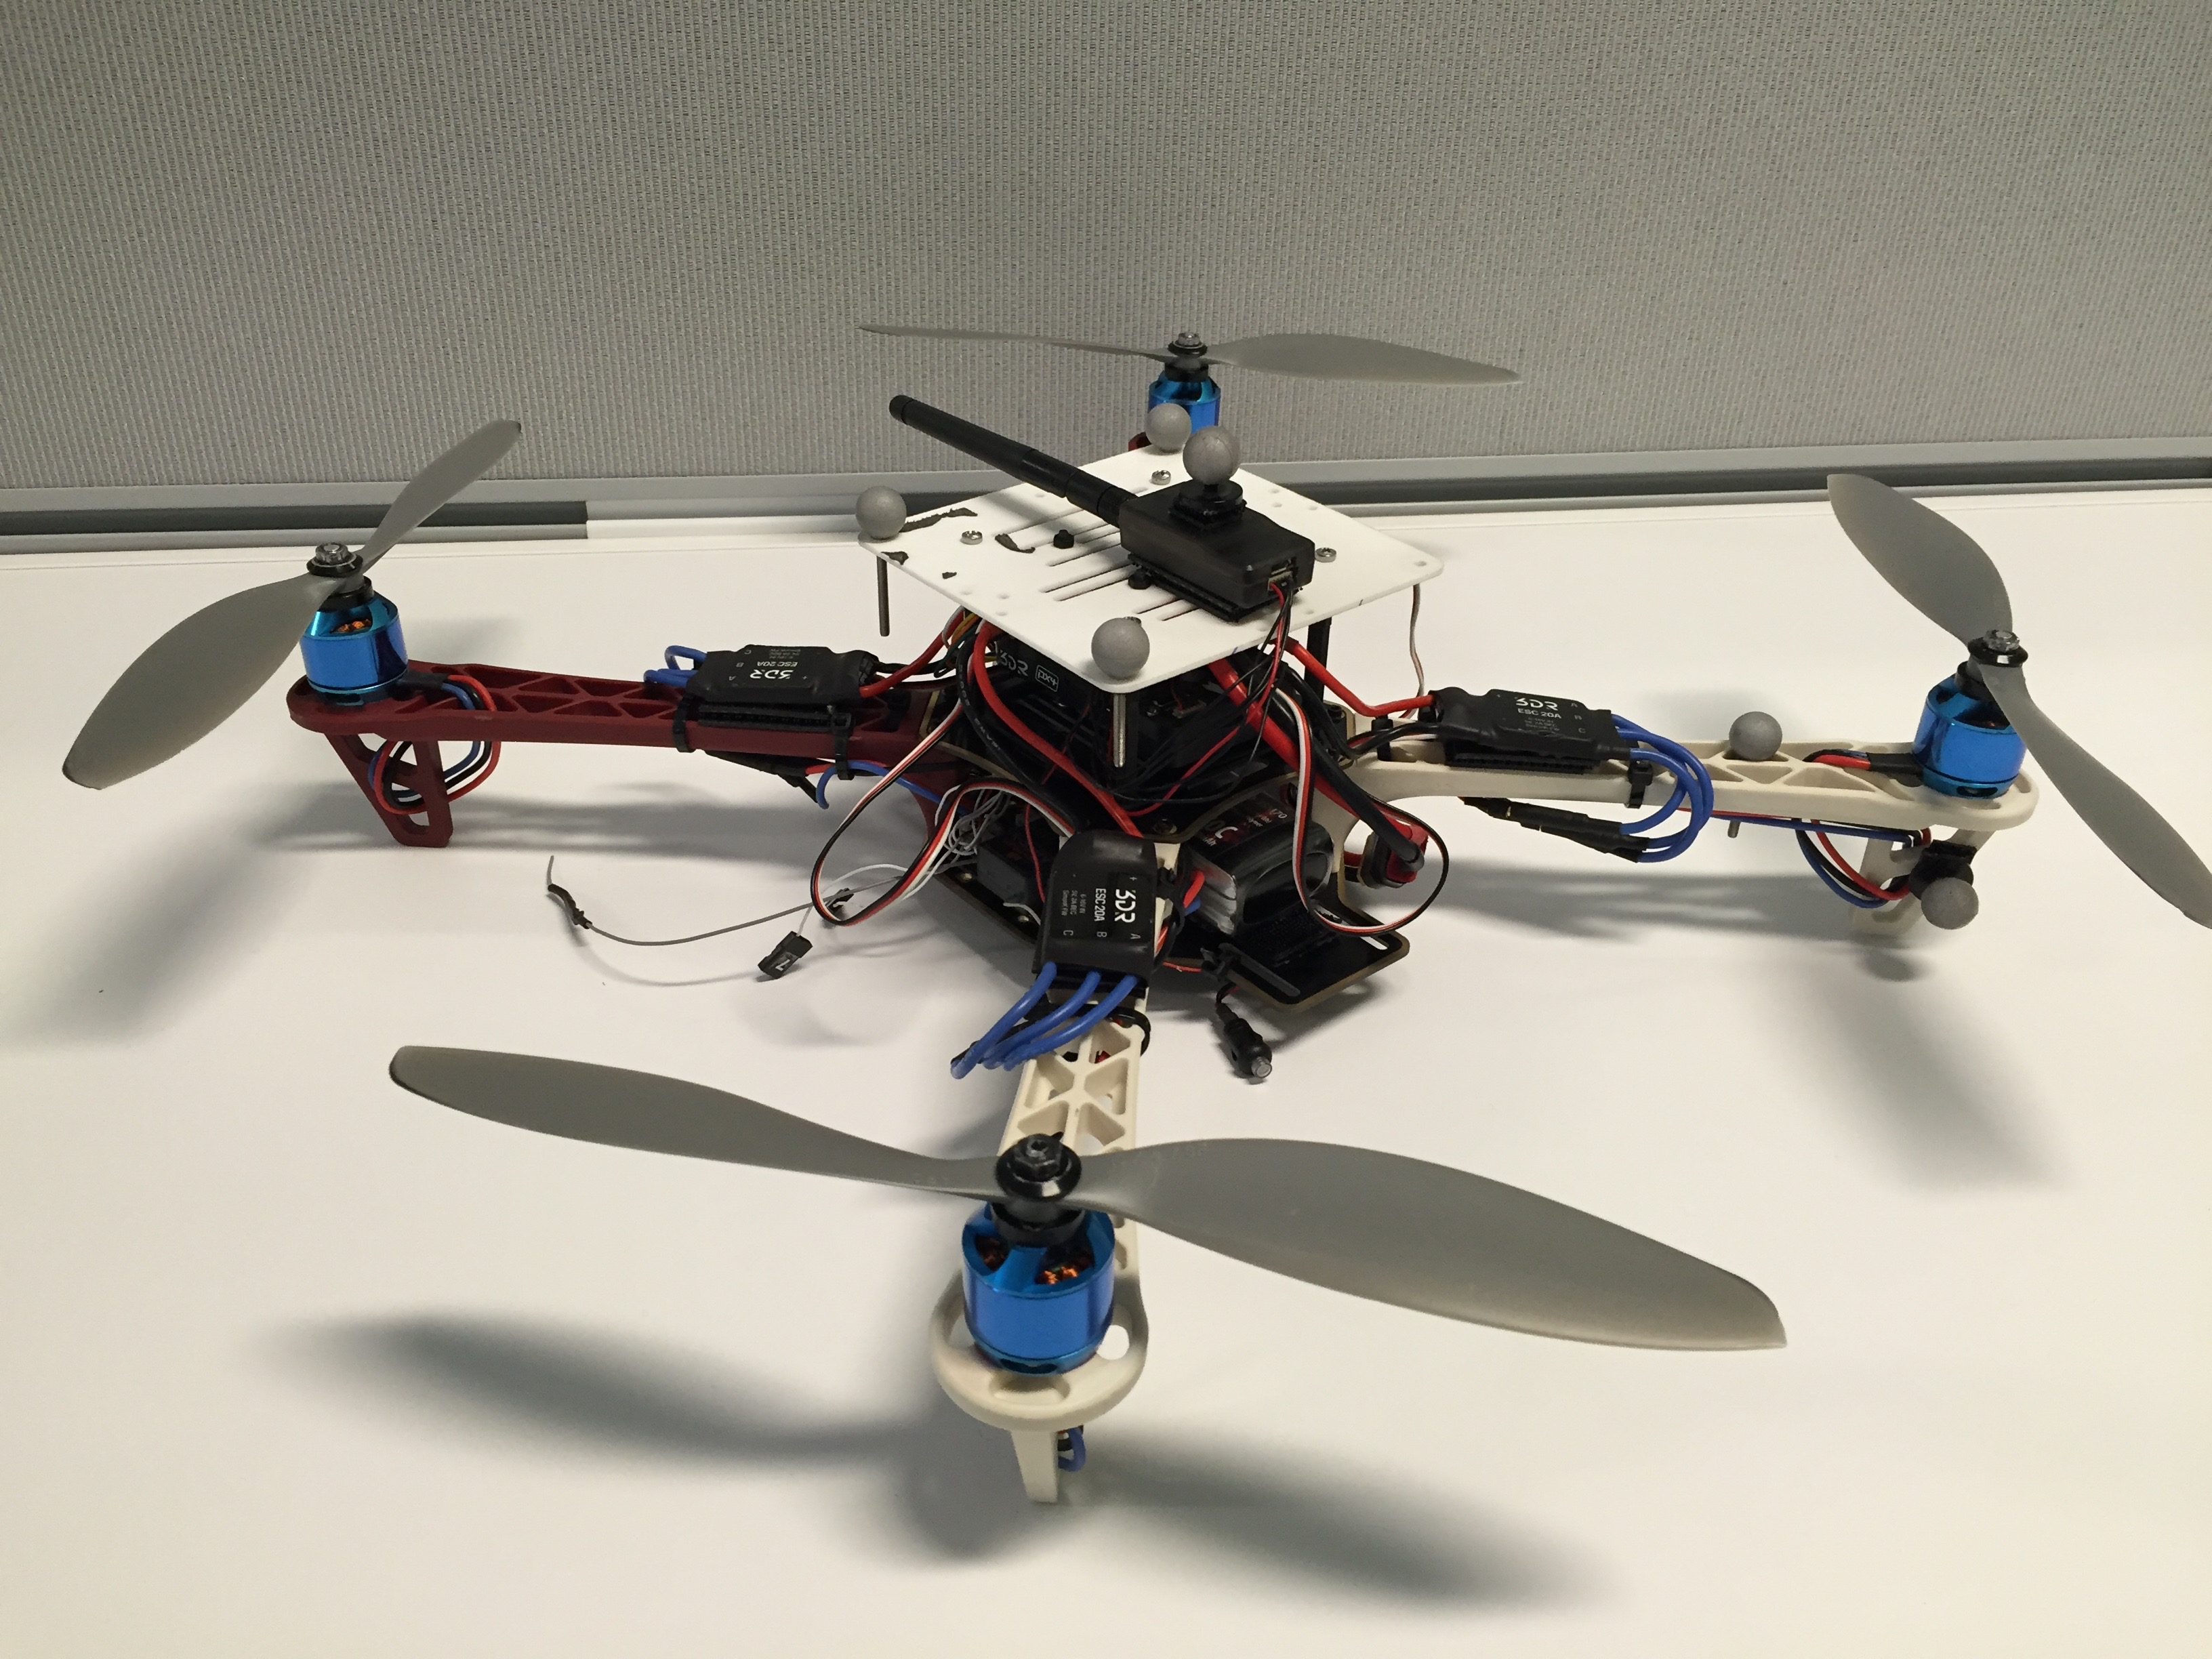
\includegraphics[width=0.8\textwidth]{graphics/quadrotor.jpg}
    \caption{Quadrotor Testbed}
    \label{fig:assemble_01}
\end{figure}

\begin{figure}
    \centering
    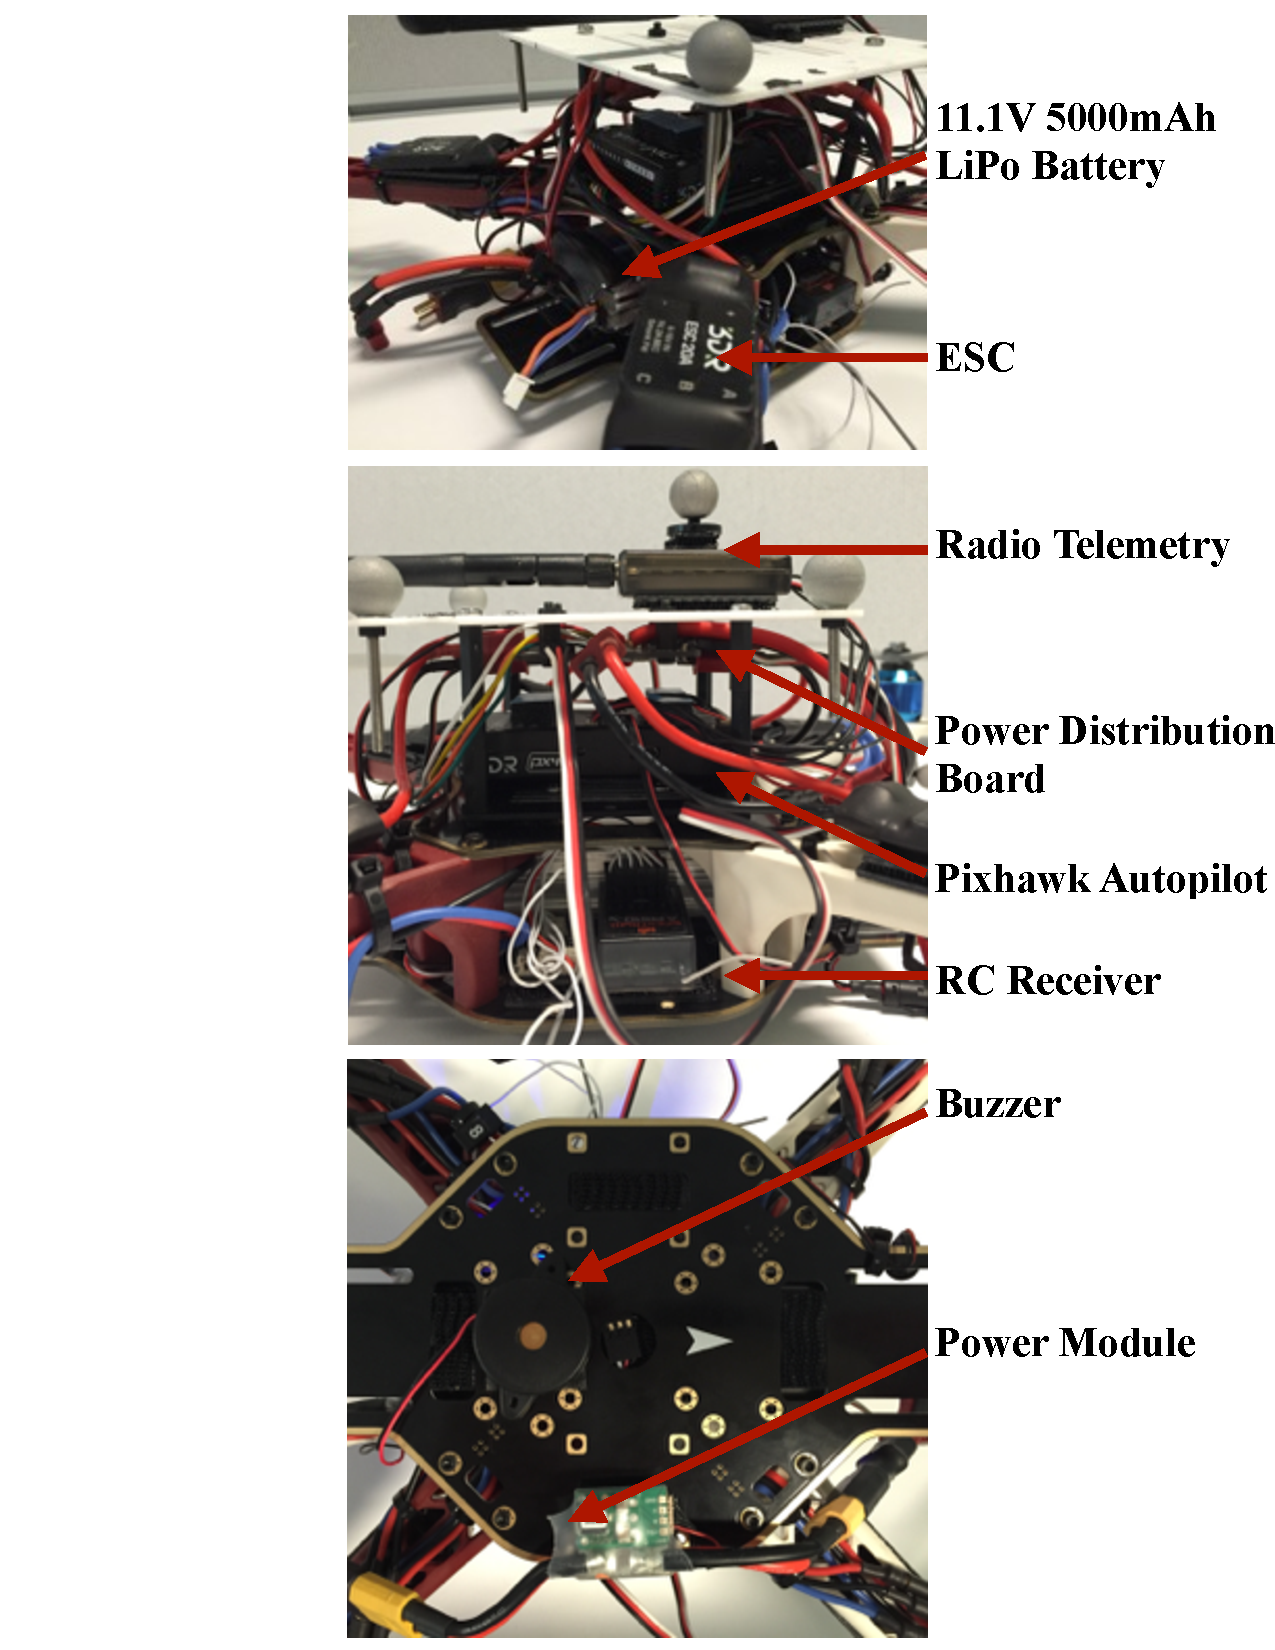
\includegraphics[width=0.9\textwidth]{graphics/hardware.pdf}
    \caption{Description of the Quadrotor Assemble}
    \label{fig:assemble_02}
\end{figure}

\begin{figure}
    \centering
    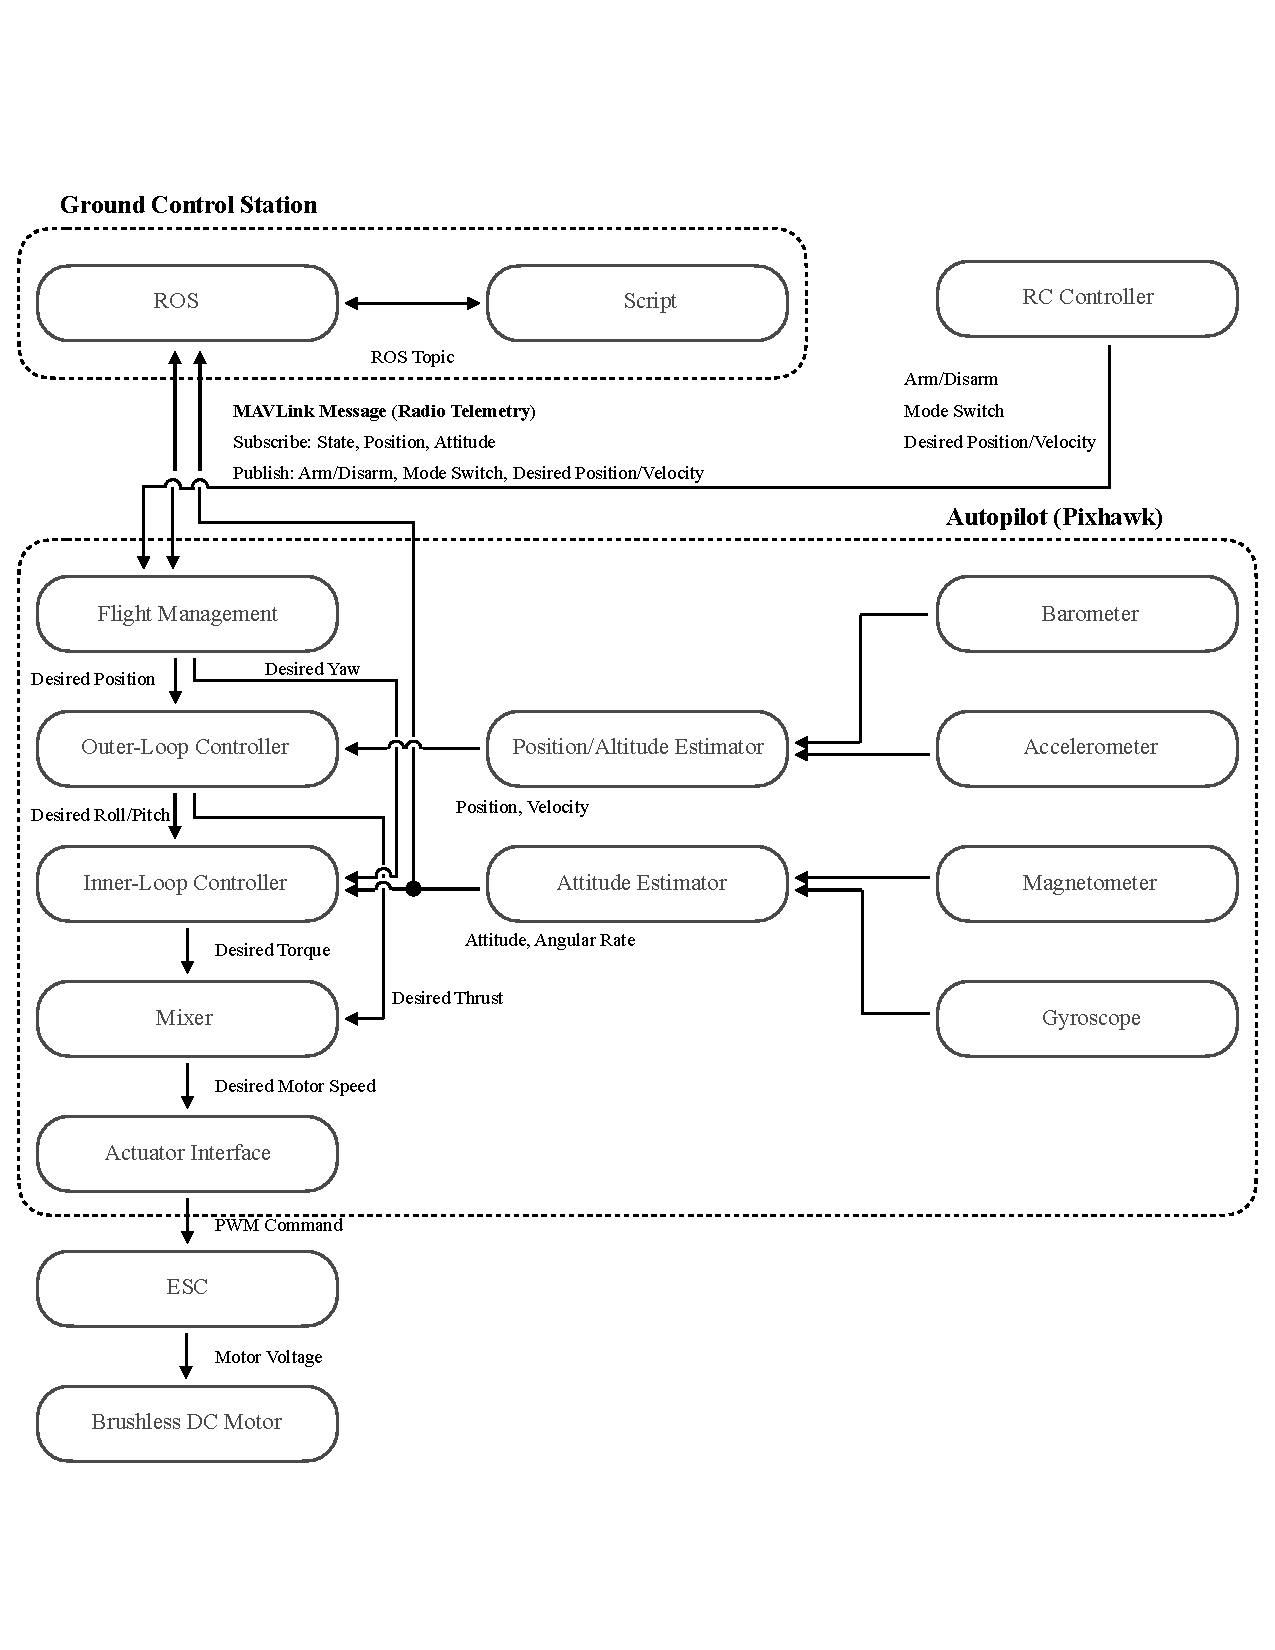
\includegraphics[width=1.0\textwidth]{graphics/architecture_01.pdf}
    \caption{System Architecture of Offboard Control}
    \label{fig:overview_01}
\end{figure}

\begin{figure}
    \centering
    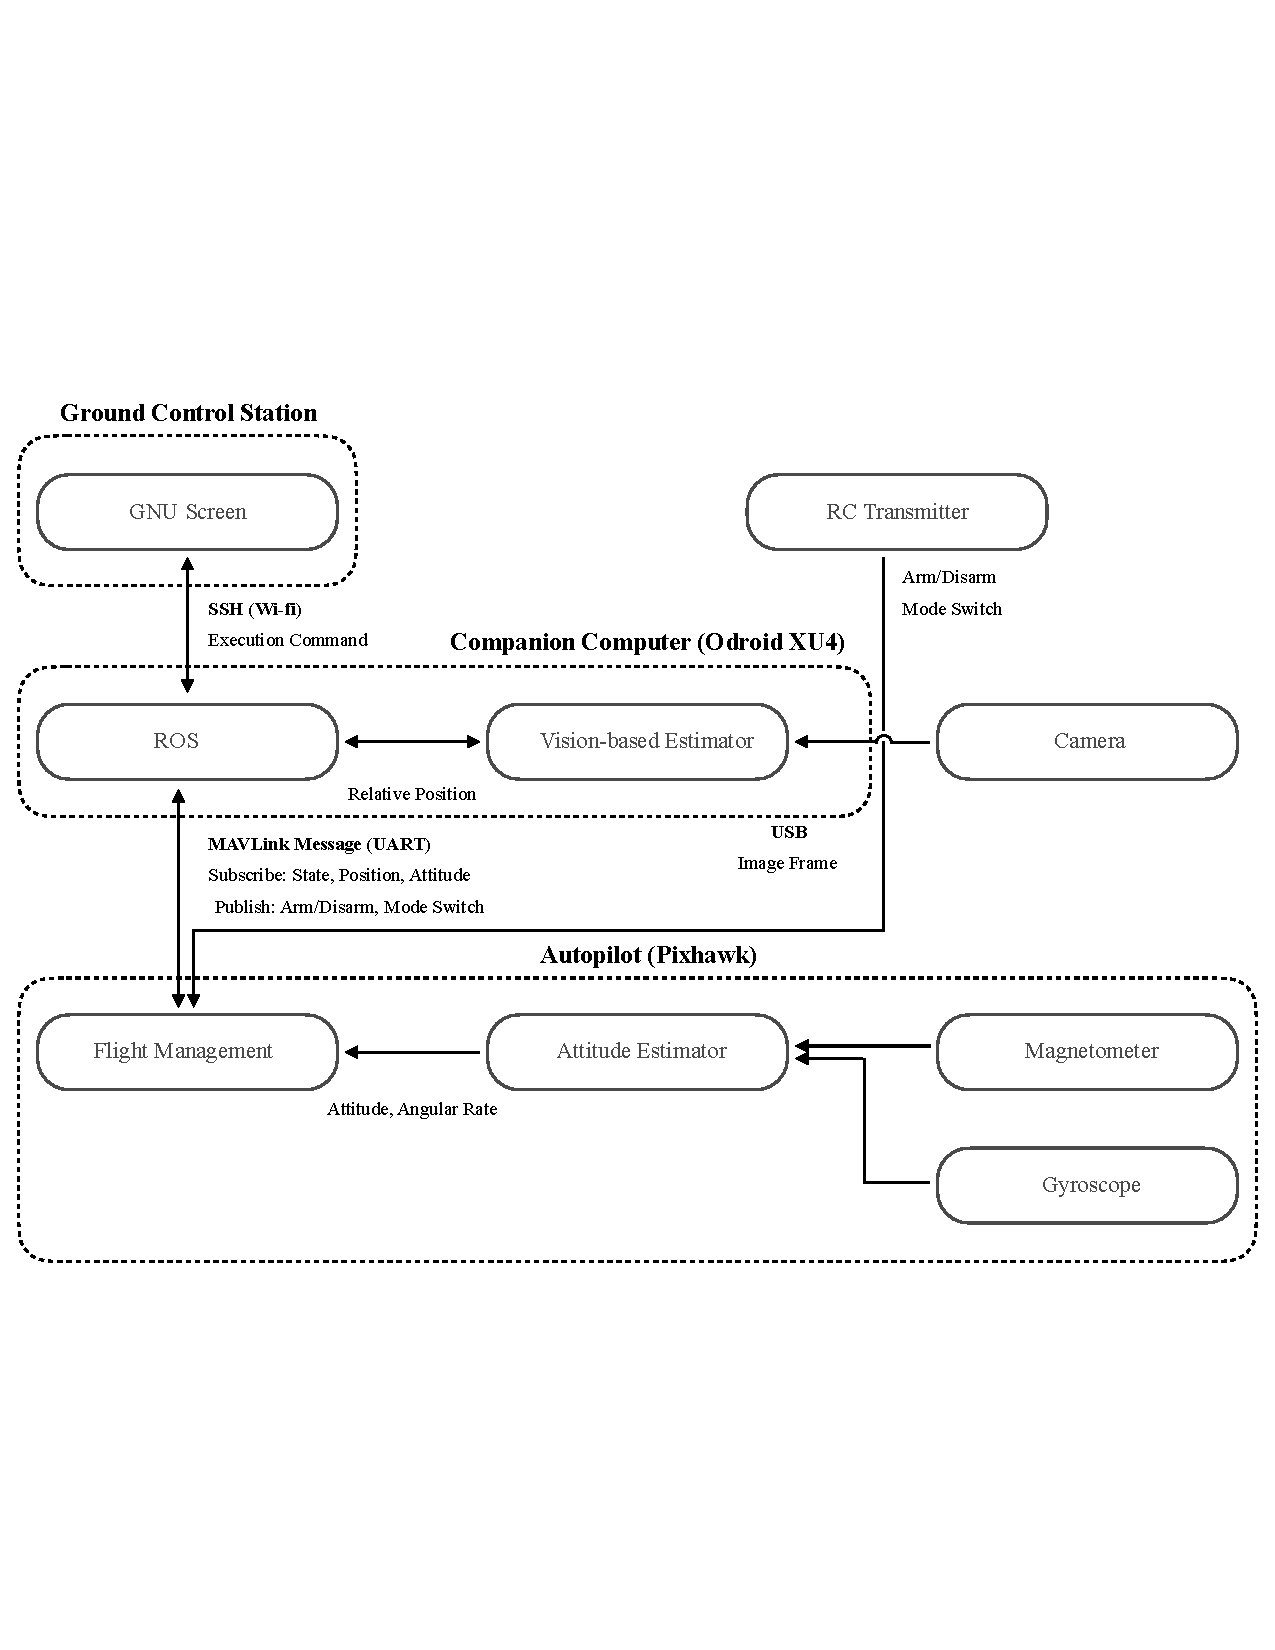
\includegraphics[width=1.0\textwidth]{graphics/architecture_02.pdf}
    \caption{System Architecture of Onboard Control}
    \label{fig:overview_02}
\end{figure}

%%%%%%%%%
In order to operate the quadrotor offboard, the quadrotor must be connected to the ground control station directly through the radio telemetries. A preprogrammed script at the ground control station sends Micro Air Vehicle Link (MAVLink) messages with control commands via radio communication between the radio telemetries stated at Subsection 2.2.8. MAVLink is a protocol that is usually used to communicate UAVs \cite{qgroundcontrol}. MAVROS, a ROS package to deal with MAVLink messages, is used to process MAVLink messages \cite{mavros}. In addition, in order for a human user to send command inputs to the quadrotor, the inputs are sent from the RC transmitter to the RC receiver. The RC receiver is directly connected to the autopilot controller.

On the other hand, the onboard companion computer estimates position information and sends command to the quadrotor, instead of the ground control station. In order to operate the quadrotor onboard, the onboard companion computer must be connected to the ground control station through a Wi-Fi network. Now the companion computer's console is available from the ground control station. Through the GNU SSH interface, the user can start and stop the autonomous operations of the quadrotor. When the autonomous operation starts, the companion computer accesses the autopilot controller and waits until the markers are in view. As soon as the ground facing camera captures the markers, the companion computer starts to estimate the position of the quadrotor. In order to estimate the position, the orientation of the camera must be known. Since the camera is fixed, the quadrotor orientation is same as the orientation of the camera and its information can be measured by the magnetometer of the autopilot. MAVLink messages are used via UART serial communication to communicate between the companion computer and the autopilot. Similar to offboard control, MAVROS is used to deal with MAVLink messages.
%%%%%%%%%
	
Once MAVLink messages are transmitted to the autopilot controller, the remaining tasks are the same in both flight control modes. However, in this research, only offboard control is used for the quadrotor flight, and onboard control is used to evaluate an onboard real-time position measurement. Therefore, the quadrotor both receives maneuver commands and exchanges the quadrotor state information in offboard control, but it only exchanges the state information in onboard control.

	There are multiple modules necessary for quadrotor flight in the autopilot: Inner-loop controller (attitude control), outer-loop controller (position control), position/altitude estimator, attitude control, and mixer. These modules are managed by a flight management system. The quadrotor's orientation, angular, rate, and acceleration are measured by the built in magnetometer, gyroscope, and accelerometer respectively. The quadrotor's position is estimated through the double integration of the acceleration and filters. The estimated altitude is corrected by the built in barometer. However, position in the other two dimensions are not corrected. As the autopilot receives MAVLink messages from the companion computer, the flight management application arms the quadrotor and starts to send setpoint data to the outer-loop controller module. Then, the outer-loop controller computes desired attitude and sends the data to the inner-loop controller module. Continuously, the inner-loop controller module computes desired torques. The mixer module receives the desired torques, computes desired motor speeds, and sends signal to the ESCs to control the motors.
	
	Open loop control is used for motor speed since the DC motors do not have encoders to measure motor speed. Instead, PWM signals are computed according to desired motor speeds to the module of the autopilot. Given PWM signals from the autopilot, each ESC controls the average voltage of its motor, which in turn controls the frequency at which the motor spins.

\section{Physical Properties}
	In order to use the dynamic model of the quadrotor, we need to know the total mass and the moment of inertia. The total mass of the assembled quadrotor is 1.404 kg. The moment of inertia is difficult to measure directly. There are two methods to estimate the moment of inertia: The first is to estimate the moment of inertia from the period of a physical pendulum. The other is to approximate the moment of inertia using a CAD model. Due to the convenience of CAD and the difficulties of installing a precise physical pendulum, we used a CAD model to estimate the moment of inertia. The origin point to compute the moment of inertia is set to be the center of the autopilot controller. The moment of inertia computed by a CAD model is given as below,\\
\begin{equation}
\begin{aligned}
J & = 
\begin{bmatrix}
J_{xx} & J_{xy} & J_{xz} \\
J_{xy} & J_{yy} & J_{yz} \\
J_{xz} & J_{yz} & J_{zz}
\end{bmatrix}\\
& = 
\begin{bmatrix}
1.206 & - 0.003318 & -0.008680 \\
- 0.003318 & 1.285 & -0.001466 \\
-0.008680 & -0.001466 & 2.347
\end{bmatrix}
\times {10}^{-2} [\textstyle{kg} {\textstyle{m}}^2]\\
\end{aligned}
\end{equation}
The diagonal elements \(J_{xx}\), \(J_{yy}\), \(J_{zz}\) are at least 150 times greater than any cross moments of inertia, the moment of inertia \(J\) is approximated as a positive diagonal matrix.\\
\begin{equation}
\begin{aligned}
J & \approx 
\begin{bmatrix}
1.206 & 0 & 0 \\
0 & 1.285 & 0 \\
0 & 0 & 2.347
\end{bmatrix}
\times {10}^{-2} [\textstyle{kg} {\textstyle{m}}^2]\\
\end{aligned}
\end{equation}
This implies that the quadrotor has a nearly symmetric structure about all axises. The components that have comparatively great mass, such as DC motors, are installed symmetrically. Even if the components that have small mass, such as the radio telemetry, are located asymmetrically, they have little effect on the moment of inertia. In addition, the battery is set close to the center of inertia, so its effect on the moment of inertia is expected to be small.

\begin{figure}
    \centering
    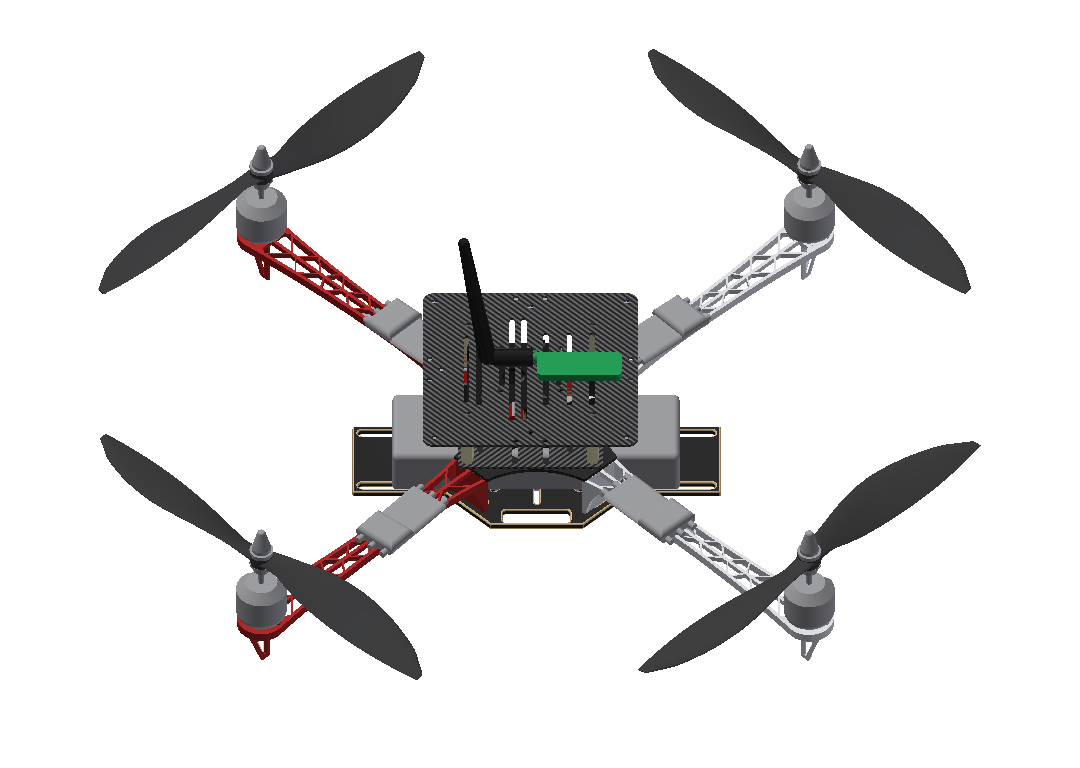
\includegraphics[width=0.6\textwidth]{graphics/cad_upper.png}
    \caption{CAD model of the Quadrotor (upper side)}
    \label{fig:cad_1}

\vspace{1cm}
    \centering
    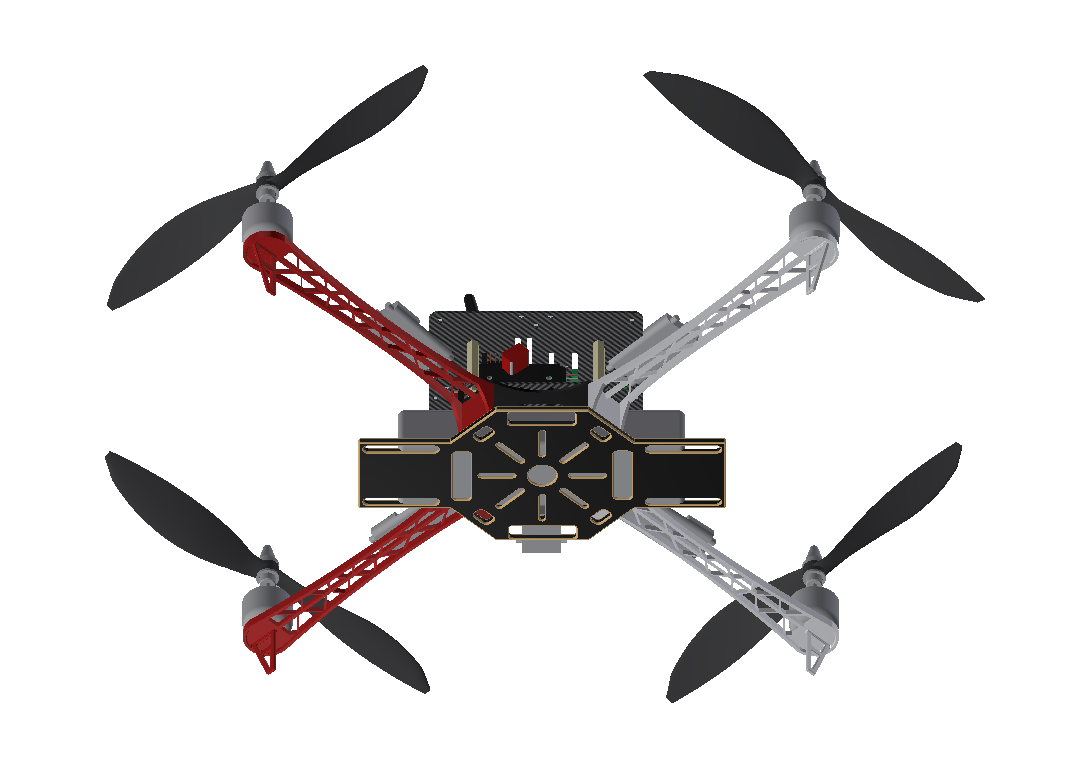
\includegraphics[width=0.6\textwidth]{graphics/cad_under.png}
    \caption{CAD model of the Quadrotor (under side)}
    \label{fig:cad_2}
\end{figure}


